\documentclass{amznotes}
\usepackage{pdfpages}
\usepackage{ctex}
\usepackage{float}
\usepackage{caption}
\usepackage{enumitem}
\usepackage{booktabs}
\usepackage{tabularx}
\usepackage{tikz}
\usepackage[svgnames]{xcolor}
\usetikzlibrary{mindmap,trees,shadows,positioning, arrows.meta}
% \usepackage{amssymb}     % 提供 \checkmark
\usepackage{lipsum}     % filler text
\newamzbox{rsbox}{结果}{result}{amztecboxcolor}
\newamzbox{ffbox}{方法}{way}{amzexboxcolor}
\newamzbox{jqbox}{渠道}{jq}{amznoteboxcolor}
\begin{document}
    \setlength{\parindent}{2em}
    
\includepdf[pages={1}]{./source/cover.pdf}
    \setcounter{tocdepth}{1}
    \tableofcontents
    \chapter{前期工作}
    \section{问卷调查}
    \subsection{调查结果}
通过发布问卷,我们初步调查了大学生信息收集的现状,得到的结果如下:
\begin{enumerate}
    \item \textbf{主要年龄段}:受调查的群体主要集中在18–22岁,占90.91\%。
    \item \textbf{主要获取信息的平台}:视频平台和搜索引擎是大学生主要的信息获取渠道,分别占36.36\%和30.91\%,这表明大学生更倾向于使用便捷且信息丰富的平台来获取信息。然而,这也从某种程度上体现出大学生在搜索时不太注重结果的可信度,尤其是视频平台的信息繁杂且难以准确检索。
    \item \textbf{信息搜索的内容}:学习相关的信息搜索占比最高,达90.91\%,这与大学生的主要任务相符合。生活困惑、活动信息等也是大学生常搜索的内容。
    \item \textbf{信息搜索的习惯}:80\%的大学生在解决问题时习惯先搜索,这说明他们在面对问题时更倾向于主动获取信息来解决。
    \item \textbf{信息搜索能力的评价}:超过半数的大学生认为自己的信息搜索能力足够,但仍有45.45\%的人认为不够,这表明部分同学在此方面还有提升空间。
    \item \textbf{信息检索能力对生活的影响}:绝大多数大学生认为信息检索能力对日常学习生活有显著影响,占比90.91\%,凸显了提高该能力的重要性。
    \item \textbf{信息检索能力不足的原因}:数据显示,缺乏检索知识及相关技能是主要原因(92\%),此外,缺少相关课程(56\%)和对设备操作不熟悉(52\%)也是重要因素;电子文盲现象普遍,许多同学在大学前未系统学习电脑操作,进一步制约了检索能力。
    \item \textbf{提高信息检索能力的方式}:开设信息素养课程(80\%)、举办信息素养讲座与培训(74\%)和参加信息实践活动(76\%)是大学生认为最有效的提升途径。
    \item \textbf{信息检索技巧的掌握情况}:只有38.18\%的大学生表示掌握一些检索技巧,多数人对技巧的了解仍较有限。
    \item \textbf{检索结果的相关性}:近一半的大学生经常遇到无法检索到理想结果或仅检索到弱相关结果的情况,说明检索精准度有待提高。
    \item \textbf{搜索结果的筛选方式}:大部分大学生会根据关键字吻合度来筛选结果(87.27\%),同时也会参考热度数据和过来人的评论。
\end{enumerate}
\subsection{拟解决方法}
根据以上调查结果,我们组思考出一下解决方法:
\begin{ffbox}{开设信息素养课程}{}

学校可以开设专门的信息素养课程,系统地教授信息检索知识和技能,如布尔逻辑检索、截词检索等技巧,以及如何使用不同的数据库和搜索引擎。对于数据库检索能力的提升尤其有必要,目前数据库是储存许多专业信息的重要形式,但许多同学甚至没有听说过数据库检索,也没有了解过一些实用的数据库。
\end{ffbox}

\begin{ffbox}{举办信息素养讲座与培训}{lecture}

学校可以邀请专业人员开展信息素养讲座和培训,介绍最新的检索工具和方法,提高大学生的信息检索意识和能力。
\end{ffbox}

\begin{ffbox}{参加信息实践活动}{comp}

组织大学生参与信息检索相关的实践活动,如信息检索比赛、科研项目中的文献检索等,增加实际操作经验。
\end{ffbox}

\begin{ffbox}{注重检索技巧的学习}{study}

大学生应主动学习和掌握各种信息检索技巧,提高检索效率和准确性。
\end{ffbox}

\begin{ffbox}{优化信息筛选方法}{}

除了根据关键字吻合度筛选结果外,还应学会结合来源可靠性、信息权威性等多种因素综合判断,提高信息质量。
\end{ffbox}
根据实践的难易程度,我们组选择进行\nameref{way:lecture}与\nameref{way:comp}作为主要活动。
    \section{采访}
    在这个信息过载的时代,检索能力已成为核心学术竞争力之一。
我们的采访所揭示的,不仅是个体的困惑,更是整个教育体系需要应对的时代命题。
我们不仅需要专业知识,更需要在大浪淘沙的信息海洋中辨别真伪、提取精华的能力。

\subsection{实操困境}
当被问及课程论文写作的第一反应时,学术数据库成为首选,这反应出我们的学生虽然知道应该使用正规学术渠道,却在实操层面面临诸多困境:
关键词搜索成为横亘在学术探索道路上的一道障碍。
"不确定自己搜的关键词对不对"、
"专业术语让人迷惑"等反馈\dots

学术数据库的检索逻辑与日常搜索引擎大相径庭、
但鲜有课程系统教学这一关键技能。
更值得玩味的是,受访者提到的"把中文关键词机翻成英文再搜索"的小技巧,
既展现了学生的创造性,也折射出工具使用教育的不足——这本应是基础技能,却成了需要自行摸索的"技巧"。

\subsection{信息渠道多元化}
值得指出的是,信息获取渠道的多元化趋势在采访中尤为明显。
短视频平台、校园论坛、经验分享会与传统学术数据库共同构成了学生的信息来源。
学生对学长学姐经验的重视反映出学术界一个长久存在的困境:隐性知识的传承往往依赖于非正式渠道。
同时,AI工具的崛起正在重塑信息检索的生态。学生对"用AI工具快速筛选文献"的强烈需求,既是对效率的追求,也隐含对传统检索方式的不满。
但关键在于,我们需要明白如何与AI协作而非依赖,如何用批判性思维审视AI提供的结果,而非全盘接受。


    \section{策划}
    \newamzbox{actbox}{活动}{activity}{amzdfnboxcolor}
对于以上结果,我们对接下来的工作进行了策划,主要分为了线上与线下两个主要的活动。
\begin{actbox}{线上电子手册编写}{books}
我们将把网络上收集到的相关信息收集技巧汇集成文档,提供一套较为完整的方法论,其中我们会按一下三个角度进行文档的编写:
\tcblower
\begin{enumerate}
    \item 科研方面的信息收集整合技巧
    \begin{notebox}
        本模块将聚焦于科研信息的高效检索与整合,
        涵盖专利检索、假新闻识别、实时科技信息获取、
        等多方面内容,
        提升同学们在科研过程中自主挖掘、筛选、评估和管理信息的能力,
        帮助同学们掌握全面获取科技动态的路径,并增强信息可靠性判断能力。
    \end{notebox}
    \item 学习相关的信息收集整合技巧
    \begin{notebox}
        本模块将聚焦于本科学习过程中信息的高效收集与整合,
        通过系统化的方法帮助同学们在海量资源中快速定位、
        筛选所需知识。

        我们将列举学习资源检索门户,并为他们排序评级,并分析途径的优缺点。
    \end{notebox}
    \item 生活相关的信息收集整合技巧
    \begin{notebox}
        本模块将会聚焦于生活方面的信息收集整合技巧,例如餐饮搜索,旅游信息收集,并给出具体案例进行分析。
    \end{notebox}
\end{enumerate}
\end{actbox}
\begin{actbox}{线下分享会举办}{share}
在线下活动方面,我们计划将我们线上所得到的知识进行宣讲与分享,并举办网络迷踪活动。
\tcblower
\begin{enumerate}
    \item 线下技巧分析(见\nameref{books})
    \begin{notebox}
        我们将所收集到的有用技巧,制作成ppt在线下进行分享。

        讲座分为三个部分,一个是为同学们接下来的科研技巧做准备的科研信息收集能力技巧分享,一个是为了同学们本科阶段学习,应考准备的学习资料信息收集能力分享,最后是
        在生活,娱乐等方面会遇到的信息收集渠道,技巧的分享。
    \end{notebox}
    \item 网络迷踪活动举行(见\nameref{activity})

    图寻是一款基于真实街景的地理知识推理游戏,
    玩家需通过观察全景图判断地点所属国家及具体位置,
    积分取决于与目标地点的距离远近。游戏通过娱乐的方式将信息收集能力,地理知识融入到游玩当中,
    兼具学习与娱乐价值。
    \begin{notebox}
        本次活动借鉴“图寻”玩法,推出“网络迷踪”挑战。
        我们将精心设计若干题目,邀请同学们发挥所学的信息检索与整合能力,在浩瀚的网络资源中快速锁定相关知识或概念,答对者即可赢取奖品,
        以此激发学习热情,提升同学们的信息素养和实战能力。
    \end{notebox}
\end{enumerate}
\end{actbox}
    \clearpage
    \chapter{电子手册}
    \label{books}
    \section{假新闻的识别和应对}
\subsection{假新闻的类型}
\begin{enumerate}
  \item 图片与视频造假

  虚假的描绘以色列与哈马斯战争的场景的照片。
  \begin{figure}[H]
    \centering
    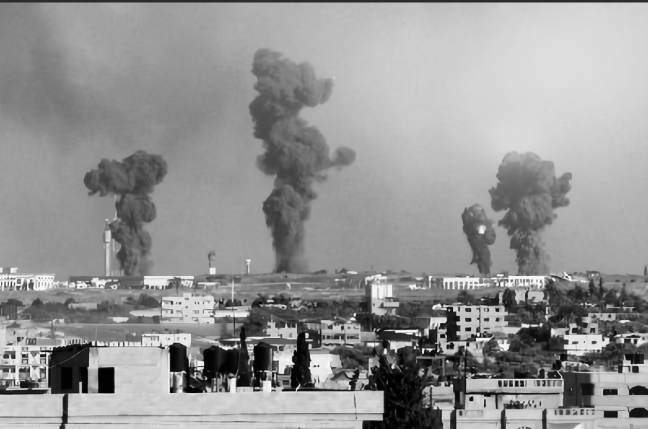
\includegraphics[width=.7\textwidth]{figures/假新闻/哈马斯.png}
    \caption{虚假战争的场景}
  \end{figure}
  \item 数据谣言

  生物学家刻意使用小样本容量,随机提供数据,只塑造关键信息,得出黑巧克力能帮忙减肥的结论。
  \begin{figure}[H]
    \centering
    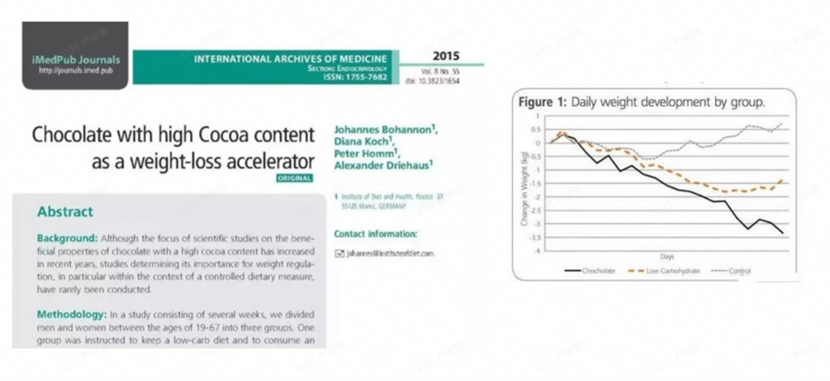
\includegraphics[width=.7\textwidth]{figures/假新闻/减肥.png}
    \caption{数据谣言}
  \end{figure}

  \item 引用作假

  通过引用所谓业内人士来作假,例如太阳报报道女王暗示支持脱欧,然而王室成员不能有任何政治倾向。
  \begin{figure}[H]
    \centering
    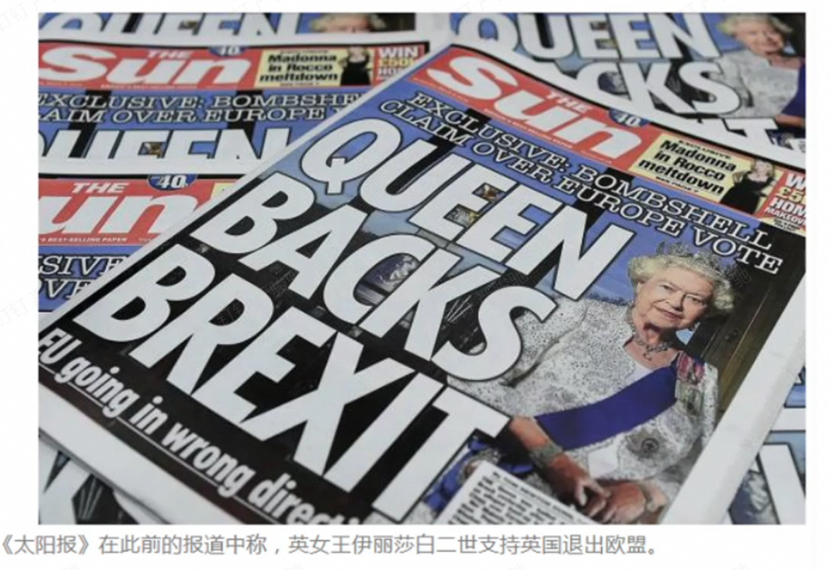
\includegraphics[width=.7\textwidth]{figures/假新闻/引用造假.png}
    \caption{引用造假}
  \end{figure}

  \item 真实的谎言

  \begin{dfnbox}{真实的谣言}{真实的谣言}
    内容大部分真实,然而在报道过程中利用模糊用词,刻意转换理解角度等手段使新闻符合读者预期
  \end{dfnbox}
  例如
  \begin{enumerate}
    \item 巴黎圣母院被大火烧毁+中国建筑师巴黎圣母院建筑竞赛夺冠$\ne$中国建筑师的这个设计方案,将会成为巴黎圣母院的重建方案。
    \item 英国的一个患癌男子感染新冠以后肿瘤消失$\ne$新冠能治愈肿瘤。
  \end{enumerate}

  \item 智能新闻
  \begin{dfnbox}{智能新闻}{智能新闻}
    完全利用AI智能生成,没有真实性
  \end{dfnbox}
\end{enumerate}
\subsection{假新闻泛滥的原因和危害}
\subsubsection{泛滥原因}
\begin{enumerate}
  \item 传播环境的影响
  \item 专业媒体竞争压力导致对核实和审查的忽视
  \item 受众的认知局限和心理特征
  \item 人工智能对虚假信息的重构
\end{enumerate}
\subsubsection{危害影响}
\begin{enumerate}
  \item 给当事人带来困扰,影响读者情绪和思维
  \item 影响新闻媒体公信力
  \item 社会秩序遭到破坏
  \item 影响国家形象
\end{enumerate}
\subsection{媒介素养与假新闻识别方法}
\begin{figure}[H]
  \centering
  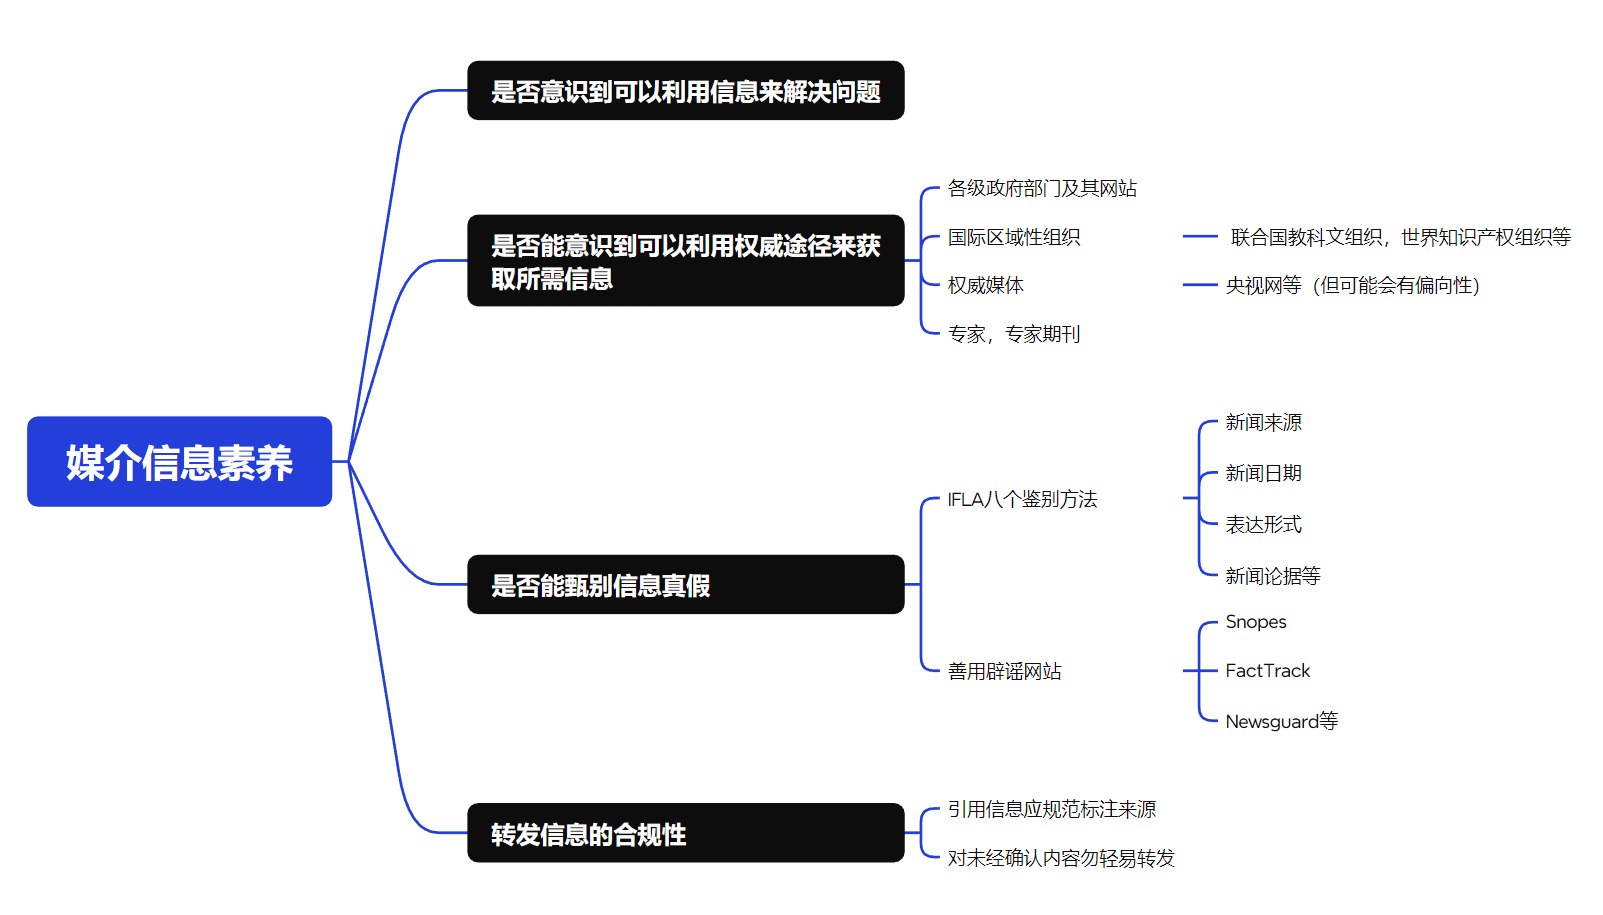
\includegraphics[width=\textwidth]{./figures/假新闻/思维导图.png}
  \caption{假新闻的应对方法}
\end{figure}
\section{科研}
\subsection{理工类文献检索方法}\label{数据库}
\subsubsection*{一、数据库选择}

\paragraph{(一)中文数据库}

\begin{enumerate}
  \item \textbf{中国知网(CNKI):} 综合性数据库,涵盖期刊、学位论文、会议论文、专利等多种文献类型,是学位论文检索的首选之一。
  \item \textbf{万方数据:} 综合性数据库,资源丰富,包含期刊、学位论文、会议论文等,适合多类型文献检索。
  \item \textbf{维普期刊:} 仅收录期刊数据,追溯年限长(从1989年起),但收录内容较杂,筛选能力弱,适合特定期刊文献检索。
\end{enumerate}

\paragraph{(二)外文数据库}

\begin{enumerate}
  \item \textbf{文摘数据库:} 对数据进行深层次加工,检索功能强大,适用于文献系统调研和优质文献筛选。常用的有:
  \begin{enumerate}
    \item \textbf{科学引文索引(SCI-E):} 基础研究首选。
    \item \textbf{科学技术会议录索引(ISTP):} 适用于应用研究。
    \item \textbf{工程索引(EI):} 适用于工程类应用研究。
    \item \textbf{Web of Science:} 涵盖多个子库,如SCI、ISTP等,是重要的外文文献检索平台。
  \end{enumerate}
  \item \textbf{全文数据库:} 更新快,适用于最新文献的补充,可在浙大图书馆数据库导航中找到。
\end{enumerate}

\subsubsection*{二、编制检索式}

\paragraph{(一)检索式定义}

检索式是使用各种符号将检索词连接起来的式子,由检索词和各种符号组成,有助于提高检索的准确性和全面性。

\paragraph{(二)检索式示例及说明}

以“人工智能和医疗”为例:

\begin{enumerate}
  \item \textbf{检索式:} \texttt{("Artificial Intelligence" OR "AI") AND ("Healthcare" OR "Medical" OR "Medicine")}
  \item \textbf{说明:}
  \begin{enumerate}
    \item \texttt{("Artificial Intelligence" OR "AI")}:用OR连接“Artificial Intelligence”和“AI”,表示文献中包含其中一个即可。
    \item \texttt{AND}:连接两个主要关键词组,确保文献同时包含人工智能和医疗相关内容。
    \item \texttt{("Healthcare" OR "Medical" OR "Medicine")}:用OR连接多个相关词汇,扩展检索范围。
  \end{enumerate}
\end{enumerate}

\paragraph{(三)检索词提取与扩充}

\begin{enumerate}
  \item \textbf{提取关键词:} 从课题的研究对象、研究目的、研究方法中提取关键词,避免使用概念过于泛化的词,如“技术”“研究”等。
  \item \textbf{扩充检索词:} 通过阅读文献综述、维基百科、Google搜索或数据库内的相关搜索扩充同义词。例如,“无线传感网”可扩充为“无线传感器网络”“传感器网络”等。
\end{enumerate}

\paragraph{(四)中文检索式编制}

以“无线传感网目标定位跟踪技术研究”为例:

\begin{enumerate}
  \item \textbf{中文检索式:} \texttt{(无线传感器网络 OR 无线传感器网 OR 传感器网络 OR 传感网络) AND 目标 AND(定位 OR 追踪 OR 检测 OR 跟踪)}
  \item \textbf{CNKI专业检索符号:} \texttt{*}表示并且,\texttt{+}表示或者,\texttt{-}表示不包含,括号表示组合。检索式可表示为:\texttt{SU=(无线传感器网络+无线传感器网+传感器网络+传感网络)*目标*(定位+追踪+检测+跟踪)}
\end{enumerate}

\paragraph{(五)英文检索式编制}

\begin{enumerate}
  \item \textbf{词组检索:} 用双引号表示,如\texttt{"sensor network"},确保检索结果中单词连在一起且位置不变。
  \item \textbf{截词符号:} \texttt{*}表示前方一致,如\texttt{object*}可检索出\texttt{objection}、\texttt{objected}等。
\end{enumerate}

\paragraph{(六)选择检索字段}

合理选择检索字段,如主题、关键词、全文、标题等,以提高检索的准确性和全面性。

\subsubsection*{三、筛选高质量文献}

\paragraph{(一)中文文献筛选}

\begin{enumerate}
  \item \textbf{综述性文献:} 优先选择综述性文献,其参考文献多、内容集中,可通过“综述”“进展”“展望”等关键词检索。
  \item \textbf{被引次数:} 被引次数高的文献通常是经典文献,可作为筛选的重要指标。
  \item \textbf{期刊筛选:} 在CNKI中可筛选北大核心期刊和CSSCI期刊,这些期刊的文献质量较高。
\end{enumerate}

\paragraph{(二)外文文献筛选}

\begin{enumerate}
  \item \textbf{数据库选择:} 优先选择Web of Science、Scopus等权威数据库。
  \item \textbf{期刊影响因子:} 关注期刊的影响因子,选择高影响因子期刊的文献。
  \item \textbf{引用追踪:} 通过文献的引用关系追踪高质量文献。
\end{enumerate}

\subsubsection*{四、特别关注}

在已知题名的情况下,可通过浙江大学图书馆首页的“求是学术搜索”检索全文,该搜索整合了图书馆的所有资源,包括纸质资源和电子资源,如期刊、图书、会议论文、报纸、政府文献等。

\subsection{开题立项前的文献调研报告}
\subsubsection*{一、为何要做文献调研}
文献调研是科研工作的基石,在开题立项前开展文献调研至关重要。它能帮助我们明确课题的研究目的、意义、作用及目标,了解前人在相关领域的研究进展,包括已取得的成果和尚存的问题,从而找准研究切入点,避免重复研究,为自身研究奠定基础并指引方向。
\subsubsection*{二、利用数据库进行文献调研}
\paragraph{选择数据库}
\paragraph{确定检索词}
\paragraph{构建检索式}
以上三部分见\nameref{数据库}。
\paragraph{查看文摘全文}
对筛选后的文献查看文摘和全文,获取详细研究内容。
若检索结果不理想,需调整检索策略,比如重新确定检索词、优化检索式等,再次进行检索,直到获得满意的结果。
\subsubsection*{三、利用 AI 搜索引擎进行文献调研}
常用的AI搜索引擎有perplexity、知乎直答、360AI搜索、秘塔AI搜索等。AI 搜索引擎信息海量但无序,默认为全文查找,查准功能相对较弱。不过,它适合检索最新文献和隐形资源,可作为专业数据库的补充,帮助我们发现一些新观点和动态,且能够直接以图表等形式生成可视化的内容,但需注意仔细筛选信息的可靠性。在使用 AI 搜索引擎时,可结合专业数据库检索结果相互印证,提高文献调研质量。
\subsubsection*{文献阅读}
\paragraph{略读}
略读时,一看题目,判断是否与研究兴趣相关;二看作者和单位,了解其学术背景,判断作者在该领域的权威性;三看摘要,明确研究问题、方法和结论;四看引言,知晓研究动机和前人主要贡献;五看正文,了解研究思路、过程和步骤;最后根据以上内容判断是否需要精读。
\paragraph{精读}
精读时,需深入分析作者及其课题组在所研究领域中的地位和贡献,明确此文在论题研究发展中的地位及作用,梳理论文的主要假设和演绎思路,剖析文献解决的关键问题和所用的基本方法的细节,总结此文的主要成绩和不足之处,最终判断此文的主要贡献及可发展的余地。在文献阅读过程中,要做好笔记,记录重要观点、数据和方法等,方便后续整理和引用。同时,要遵循学术论文(著作)的引用规范,如果违反相应的条例会受到学校的处罚。
\subsubsection*{四、学术论文(著作)引用规范}
\begin{enumerate}
  \item 引用范围界定

  只引用公开发表的文献,确保引用来源的可靠性与可追溯性。公开发表文献经过同行评审等流程,在内容准确性和科学性上更有保障。

  \item 引用原始文献

  优先引用原作者的原始文献和第一手资料,直接获取最准确的研究成果和观点阐述,避免因引用二次文献产生信息偏差。例如在引用实验数据时,直接引用原作者发表的实验报告,而非他人对该实验的解读。

  \item 合作成果引用标注

  引用合作者的观点或研究成果时,必须加注说明,尊重合作者知识产权,明确贡献归属。

  \item 转引规范

  转引他人成果既要注明转引出处,又要注明原文出处,保证文献引用链条完整清晰,方便读者追溯原始文献。

  \item 特殊内容引用

  模型、图表、数据也应注明出处,这些元素可能是原作者研究成果重要组成部分,注明出处是对知识产权的尊重,也增强自身论文可信度。

  \item 著录格式标准化

  采用标准化的著录格式,如 APA、MLA、GB/T 7714 等格式,不同学科领域可能有推荐格式,严格按照格式要求著录文献信息,使论文参考文献部分规范、统一,便于读者查阅。

\end{enumerate}
\section{本科阶段的学习}
由于信息的多元化导致信息搜索易迷失方向,发生低效搜索的情况,而且部分同学缺少获取信息的途径以及方法,
在这个章节,我们希望通过集合多种方法帮助同学们了解各种获取信息的渠道,将各种渠道进行整合和分析。
\begin{jqbox}{CC98\&朵朵}{}
    最常用的两个学校论坛
    \tcblower
    \begin{enumerate}
        \item \textbf{优点:}可以在其中发现许多历年卷、教材答案等各种学习资料以及最新的消息,
        拥有多方面的学校内的信息,打破同学间的信息壁垒。
        \item \textbf{缺点:}可能需要投入一定的时间,搜索过程缺乏有效关键词。
    \end{enumerate}
    相关历年卷可以在CC98的\textbf{学习天地}板块进行搜索,相关专业课可以去学院专版进行搜索。

    云朵朵中本科,尤其是大一的用户居多,可以在论坛上发起相关讨论形成良性的讨论圈。
\end{jqbox}
\begin{jqbox}{老师\&同学}{}
    可以提供情感价值的解答问题好友
    \tcblower
    \begin{enumerate}
        \item \textbf{优点:}较为灵活的获取信息解答问题的途径,有效解决实时问题。
        \item \textbf{缺点:}或许会有“已读不回”以及难以解决问题的情况而造成一些尴尬。
    \end{enumerate}
\end{jqbox}

\begin{jqbox}{DeepSeek等AI}{}
    新兴产生的好途径
    \tcblower
    \begin{enumerate}
        \item \textbf{优点:}依托大数据为背景,聚集各种知识要点。
        \item \textbf{缺点:}可能会出现知识错误以及误导,需要增强判断和甄别能力。
    \end{enumerate}
\end{jqbox}

\begin{jqbox}{知乎}{}
    当前解决问题的一个大网站
    \tcblower
    \begin{enumerate}
        \item \textbf{优点:}获取许多前辈们的资源与避雷指南,评论区常有深度交流。
        \item \textbf{缺点:}部分文章过长,信息冗余,需要耐心筛选。
    \end{enumerate}
\end{jqbox}

\begin{jqbox}{百度\&夸克}{}
    大功能性网站
    \tcblower
    \begin{enumerate}
        \item \textbf{优点:}获取全方位的资源,打破校区与国家壁垒,拥有大量实时消息。
        \item \textbf{缺点:}信息参差不齐,部分内容需充值会员或质量难以保证。
    \end{enumerate}
\end{jqbox}

\begin{jqbox}{QQ\&微信\&钉钉答疑群}{}
    校内或校外的分享思考之地
    \tcblower
    \begin{enumerate}
        \item \textbf{优点:}通过探讨共同进步,可搜索已提交的问题并获取他人经验。
        \item \textbf{缺点:}群内人员复杂,可能得不到及时或专业的帮助。
    \end{enumerate}
\end{jqbox}

\begin{jqbox}{微信公众号}{}
    获取学习资料的便捷途径
    \tcblower
    \begin{enumerate}
        \item \textbf{优点:}可获得前辈们整理的学习资料和经验分享。
        \item \textbf{缺点:}覆盖学科有限,资源更新不够及时,内容深度参差不齐。
    \end{enumerate}
\end{jqbox}

\begin{jqbox}{B站}{}
    获得各地学习视频的主流平台
    \tcblower
    \begin{enumerate}
        \item \textbf{优点:}丰富的视频讲解与题目演示,多样化学习思路。
        \item \textbf{缺点:}知识点不一定全面,与校内课程难度不完全匹配。
    \end{enumerate}
\end{jqbox}
值得一提的是,现在针对本科生学业问题,各大学园也在持续发力,例如蓝田的学长答疑室,云峰的学业加油站等。

总结:搜索信息注重精准性,根据所要搜索的信息类别确定搜索的方式,并且注重权威性,
通过正当的渠道获取正确的信息,最后,注意全面性,全方位的思考获取的资源的可靠性。

\section{生活娱乐等}
\subsection{旅游信息收集}
\subsubsection{搜索平台}
\begin{enumerate}
  \item 综合性旅游平台(提供景点、酒店、交通一站式服务):携程、飞猪、去哪儿。
  \item 攻略分享平台(用户生成内容,含详细行程和避坑指南):马蜂窝、穷游网。
  \item 社交媒体(获取最新体验和避雷建议等):小红书、抖音、哔哩哔哩。
  \item 地图类工具(查看景点开放时间、门票、用户评价):高德地图、百度地图。
  \item 各地文旅局官网/公众号(获取权威信息,查看黑名单):杭州市文化广电旅游局、乐游上海等。
\end{enumerate}
\begin{figure}[H]
\centering
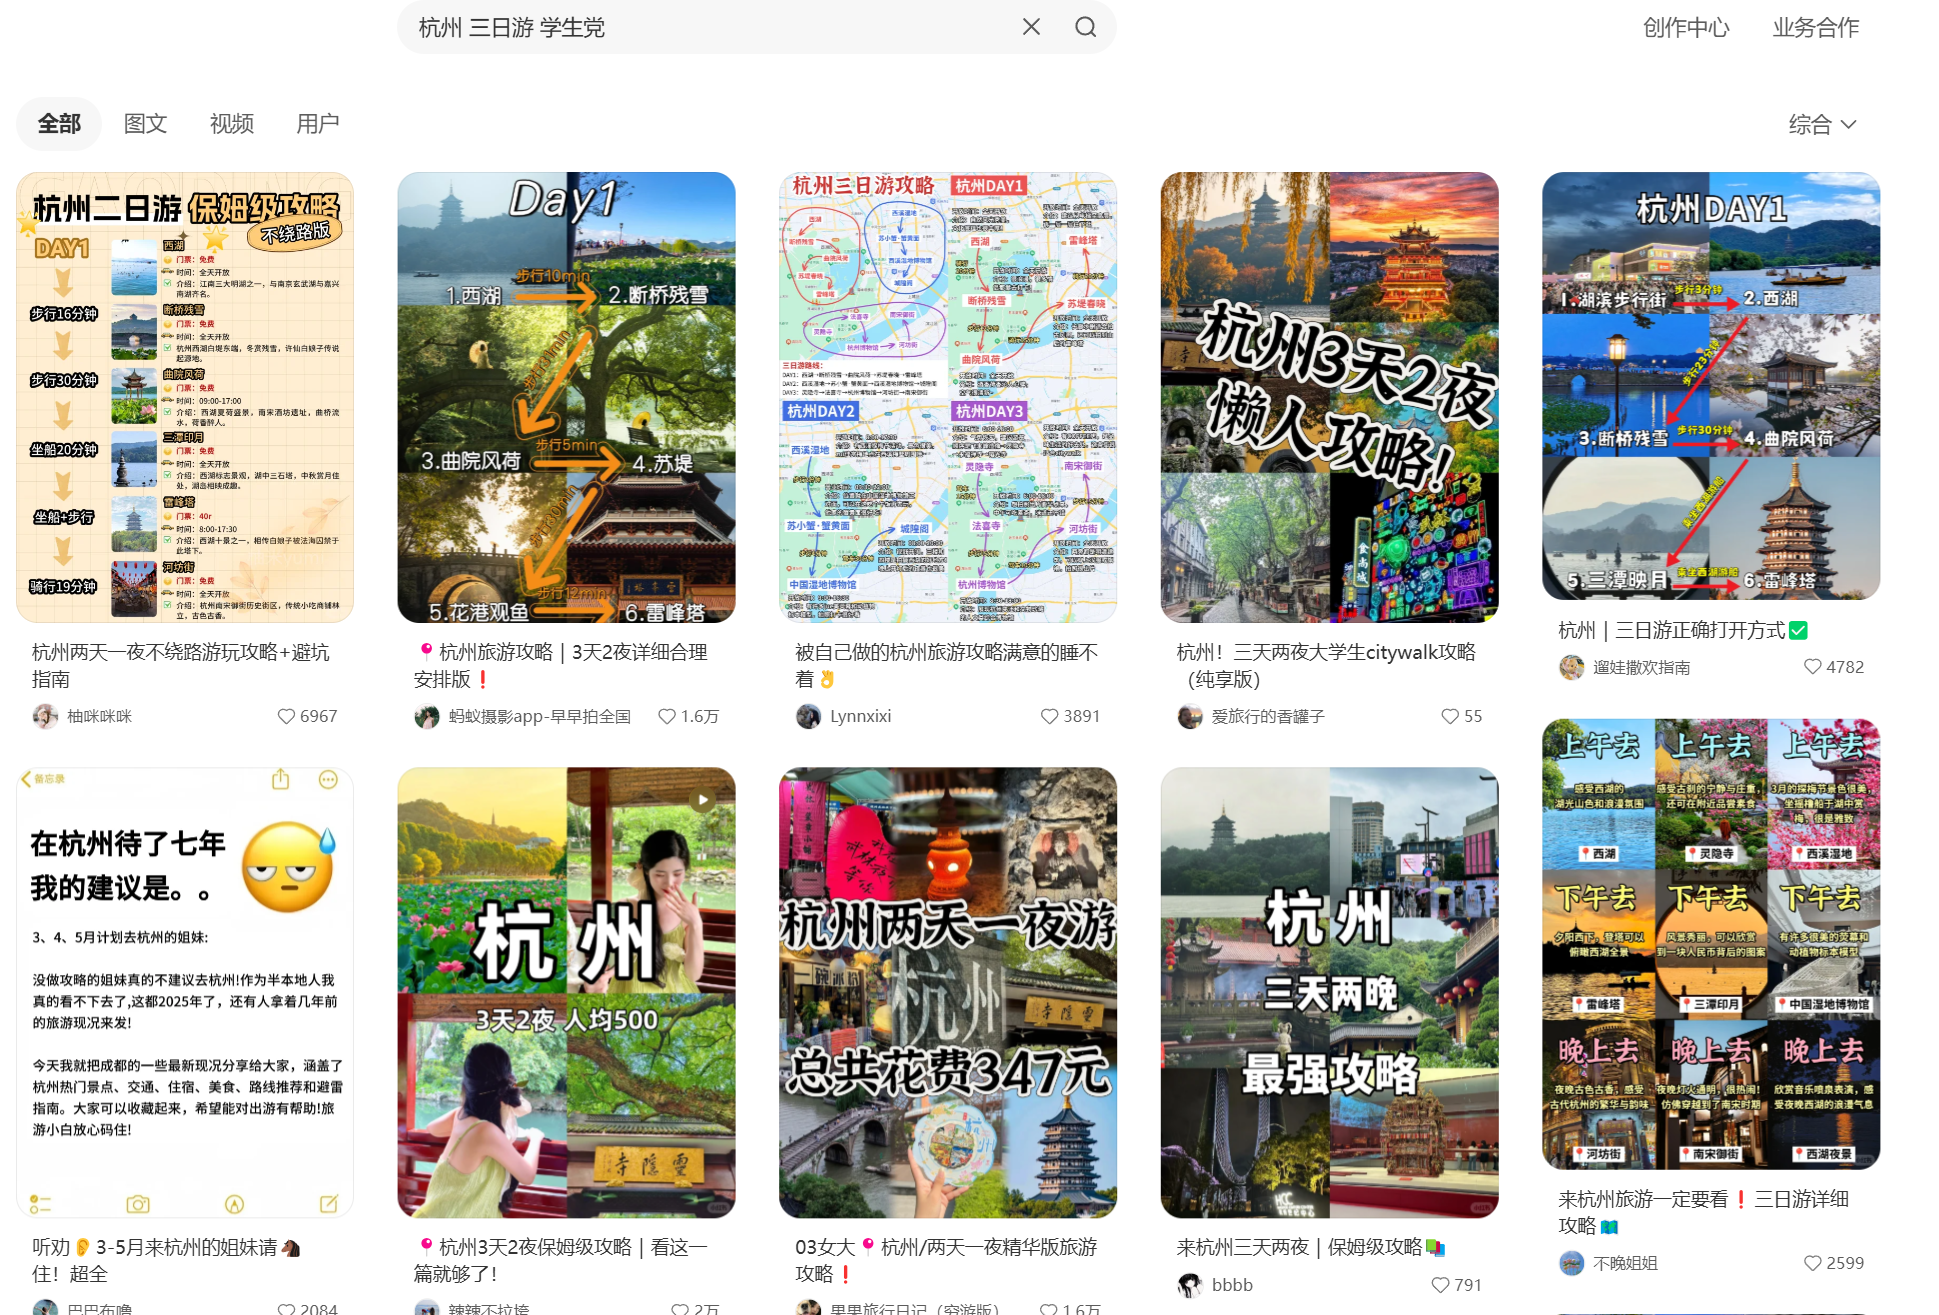
\includegraphics[width=.8\textwidth]{./figures/生活/示例1.png}
\caption{搜索示例}
\end{figure}
\subsubsection{搜索技巧}
\begin{enumerate}
  \item 关键词组合:如“杭州 三日游 学生党”,“重庆 美食打卡 5月”
  \item 避坑话术:如“XX景点 不要去”
  \item 筛选条件:优先选择“最新发布”“高赞笔记”等,避开广告软文
\end{enumerate}
\subsubsection{进阶搜索技巧}
\begin{enumerate}
  \item 双引号“”  :强制完全匹配短语,避免拆分或谐音干扰
  \item 减号-    :排除含特定关键词的页面,适用于过滤广告或无关内容。
  \item 通用支持:""、-、site:、filetype:、inurl:、intitle: 等指令适用于Google、Bing、百度等主流搜索引擎。
  \item 部分支持:allintitle:在百度中可能失效,建议拆分为intitle:多关键词组合使用。
\end{enumerate}
\begin{figure}[H]
  \centering
  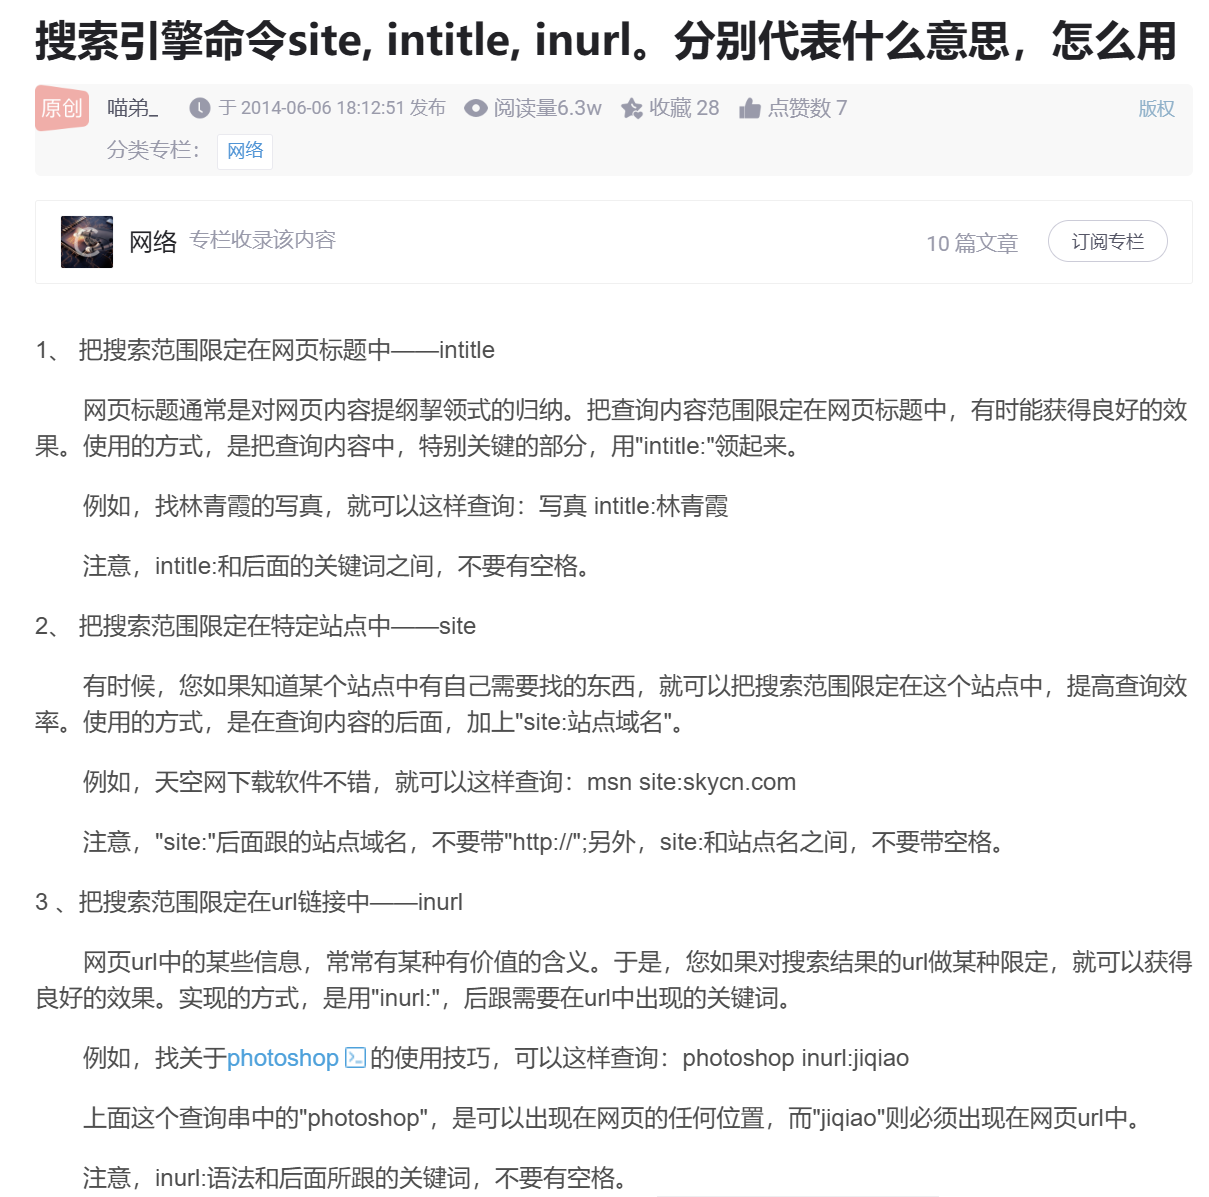
\includegraphics[width=.8\textwidth]{./figures/生活/示例2.png}
  \caption{搜索进阶}
\end{figure}
\begin{exbox}{进阶搜索实例}{advanced search}
  \begin{itemize}
    \item "迪士尼门票折扣" -广告 -推广 intext:2025

    \item intitle:"西湖 醋鱼" intitle:老字号

    \item 限定网站:关键词 site:网站域名(排除非垂直平台信息,提升可信度):如“重庆火锅 site:dianping.com”
  \end{itemize}
\end{exbox}
\subsubsection{学生特惠}
\begin{enumerate}
  \item 支付宝
  \begin{enumerate}
    \item 校园派:集中展示学生专属红包、任务奖励、品牌联名优惠(如餐饮折扣、出行券包)
    \item 学生特惠:长期展示学生专属折扣商品、生活服务优惠。
  \end{enumerate}
  \begin{figure}[H]
    \centering
    
\includegraphics[width=.8\textwidth]{./figures/生活/学生优惠_支付宝.png}
    \caption{支付宝学生优惠}
  \end{figure}
  \item 12306
  \begin{enumerate}
    \item 票价优惠
  \end{enumerate}
  \begin{figure}[H]
    \centering
    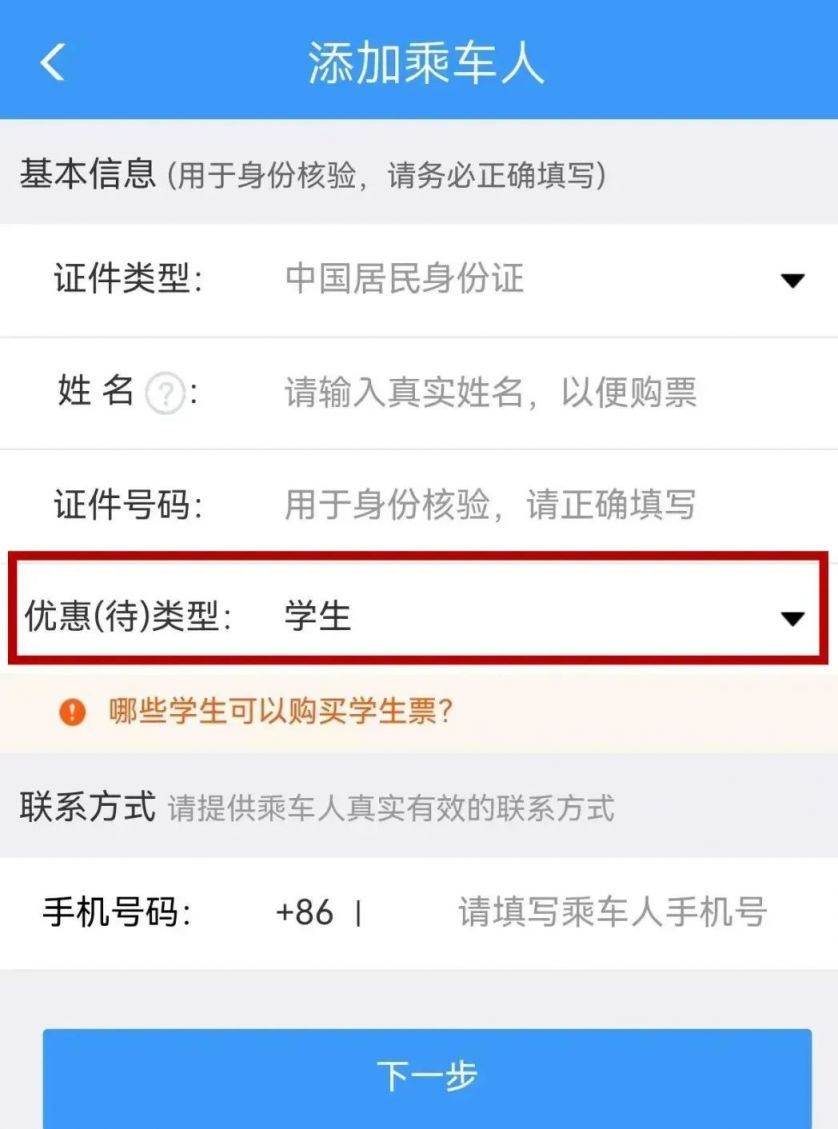
\includegraphics[width=.8\textwidth]{./figures/生活/学生优惠_12306.jpg}
    \caption{12306学生优惠}
  \end{figure}
  \item 美团
  \begin{enumerate}
    \item 学生专属红包/神券
    \item 返校优惠/交通票务折扣
    \item 学生价/首单优惠
  \end{enumerate}
\end{enumerate}
\subsection{餐饮信息收集}
\subsubsection{搜索平台}
\begin{enumerate}
  \item 外卖平台(查看商家评分、用户评价、优惠活动):美团、饿了么
  \item 生活平台(筛选“高校周边”“学生推荐”标签):大众点评
\end{enumerate}
\subsubsection{搜索技巧}
\begin{enumerate}
  \item 关键词组合:「口味+价格」,「品牌+活动」等
  \item 筛选条件:筛选距离,好评,价格区间,用餐场景等等
\end{enumerate}
\textbf{餐饮类重点关注:卫生情况,口味评价,口碑评分等}
\subsubsection{卫生情况}
\begin{enumerate}
  \item 查看证照信息(操作路径:商家页面 → 资质公示 → 食品经营许可证 )

  在商家页面进入「商家信息」或「资质」板块,重点查看公示的食品经营许可证。持有该证照的商家通常具备固定营业场所,

  \item 查看卫生评级

  部分城市在美团平台标注商家卫生评级(如A/B/C级),优先选择A级或B级商家,此类商家卫生状况更可靠。

  \item 观察环境图片

  商家页面展示的店铺实景图可直观反映堂食环境。若图片包含桌椅、用餐区等元素,则说明支持堂食;若仅展示后厨或打包区,可能为纯外卖店铺。

  \item 分析用户差评

  重点筛选差评中的卫生相关关键词,如“吃出异物”“蟑螂”“油污”“食材不新鲜”等。若差评集中反映卫生问题,需谨慎选择。

\end{enumerate}
\subsubsection{口碑评分}
\begin{enumerate}
  \item 查看综合评分

  商家页面顶部显示星星数量评分,星星越多代表综合口碑越好。评分基于口味、环境、服务、配送等多维度计算。

  \item  筛选用户评价标签(操作路径:评价区域 → 筛选 → 选择标签类型 )

  在评价区域,可通过筛选功能查看好评、差评或有图评价。美团还提供标签化分类,如“味道赞”“分量足”“服务好”等,快速定位高频评价点

 \item  分析评价内容

  \begin{enumerate}
    \item 好评参考:关注用户对菜品口味、服务态度、环境舒适度的具体描述。
    \item 差评警惕:若差评集中在菜品质量、卫生问题或服务态度,需结合其他信息综合判断。
  \end{enumerate}
\end{enumerate}
\subsection{娱乐场所信息收集}
\subsubsection{搜索平台}
\begin{enumerate}
  \item 娱乐类平台(查询演出、电影、展览信息):猫眼、大麦
  \item 生活平台(查看KTV、台球馆、密室逃脱评分) :美团、大众点评
  \item 校园社群(获取学长学姐推荐的“宝藏店铺”):校园墙/朵朵校友圈
\end{enumerate}
\textbf{娱乐场所类重点关注:安全情况,卫生情况,体验情况等}
\subsubsection{评估安全性}
\begin{enumerate}
  \item 官方在线查询平台
  \begin{enumerate}
    \item 国家企业信用信息公示系统

    查询方式:登录系统官网,输入场所名称或统一社会信用代码,即可获取企业登记信息,包括营业执照状态、经营范围、法定代表人等。

    \item 地方政务服务平台

    查询方式:部分地区提供本地化查询服务(如北京通APP的“娱乐场所营业资格查询”功能),可结合企业信用信息公示系统使用。
  \end{enumerate}
 \item 实地核查
 \begin{enumerate}
  \item 显性标识检查
  \begin{itemize}
    \item 法律依据:根据《中华人民共和国公司法》,营业执照正本应置于经营场所醒目位置。
    \item 操作要点:尽量选择连锁品牌,直接前往场所,查看是否在显眼位置悬挂营业执照,并核对信息是否与场所名称、地址一致。
  \end{itemize}
  \item 证照公示情况

  除营业执照外,娱乐场所还需公示《娱乐经营许可证》等专项许可文件。若场所无法提供或公示信息不完整,可能存在违规经营风险。
 \end{enumerate}
 \item 官方渠道核实

 工商行政管理部门/文化市场监管部门咨询核查

 拨打当地工商部门或文化市场监管部门咨询电话,或前往办事窗口,提供场所名称、地址等信息,申请查询其证照核发和年检状态。

 \item 第三方数据平台

 \begin{enumerate}
  \item 企查查/天眼查

  输入场所名称,查看其关联风险(如行政处罚记录、司法诉讼),曾因不达标/不合规被罚款的场所可能存在安全隐患。
  \item 消费投诉平台
         \begin{itemize}
          \item 12315平台:查询场所投诉量及解决率,高频投诉问题(如“强制消费”“中途加价”)需重点警惕。
          \item 黑猫投诉:搜索场所名称,关注用户上传的交易凭证(如消费小票、聊天记录)
         \end{itemize}
 \end{enumerate}
\end{enumerate}
\subsubsection{卫生情况}
\begin{enumerate}
  \item 公示文件核查:查看场所是否悬挂《公共场所卫生许可证》,有效期通常为4年,需确认是否在有效期内。
  \item 环境细节观察:
         \begin{enumerate}
          \item 包厢清洁:桌面、地面无杂物水渍,沙发/皮凳无污渍,踢脚板无灰尘。
          \item 设备卫生:麦克风球套定期更换,麦克风头无损坏,点歌面板无灰尘。
          \item 公共区域:卫生间面盆、浴缸、坐便器每客一消毒,无积水、污垢或异味;垃圾桶及时清倒,垃圾袋及时更换
         \end{enumerate}
  \item 卫生等级参考
        \begin{enumerate}
          \item \item 部分地区对娱乐场所进行卫生评级(如A级优秀、B级良好、C级一般),可通过当地卫生监督部门官网查询场所评级信息。  3. 卫生检测报告
         \item 正规场所应定期进行空气质量、水质、噪声等检测,并公示检测报告。可要求场所提供近期检测报告,重点关注甲醛、二氧化碳、细菌总数等指标是否达标。
        \end{enumerate}
\end{enumerate}
\subsubsection{口碑情况}
\begin{enumerate}
  \item 主流消费平台
  \begin{enumerate}
    \item 美团/大众点评:

    通过搜索KTV名称查看综合评分(满分5分)及用户评价标签(如“音效好”“服务热情”)。

    重点关注高频差评关键词,如“设备故障”“服务冷漠” “曲库更新”“隔音效果”“包厢卫生”等,可直观反映实际体验。
    \item 带图评价:用户上传的包厢环境、设备状态等照片,可辅助判断场所条件。
  \end{enumerate}

  \item 垂直领域平台
        \begin{enumerate}
          \item 小红书/抖音/哔哩哔哩:关注博主探店视频中的音效测试、卫生细节、套餐性价比分析。
          \item 本地/校园生活论坛:获取居民/朋辈对场所的长期口碑反馈
        \end{enumerate}
  \item 社交媒体舆情监测
  \begin{enumerate}
    \item 微博超话/话题
    \item 微信生态(公众号/朋友圈)
  \end{enumerate}
\end{enumerate}
\subsection{案例分享}
\begin{exbox}{挑选校园附近KTV}{KTV}
  通过四种途径,展示挑选校园附近KTV的方法
  \tcblower
  \begin{enumerate}
    \item 小红书搜索筛选

    组合关键词搜索+排序标签筛选+评论查看(并关注点赞,收藏数)

    锁定门店候选
    \begin{figure}[H]
      \centering
      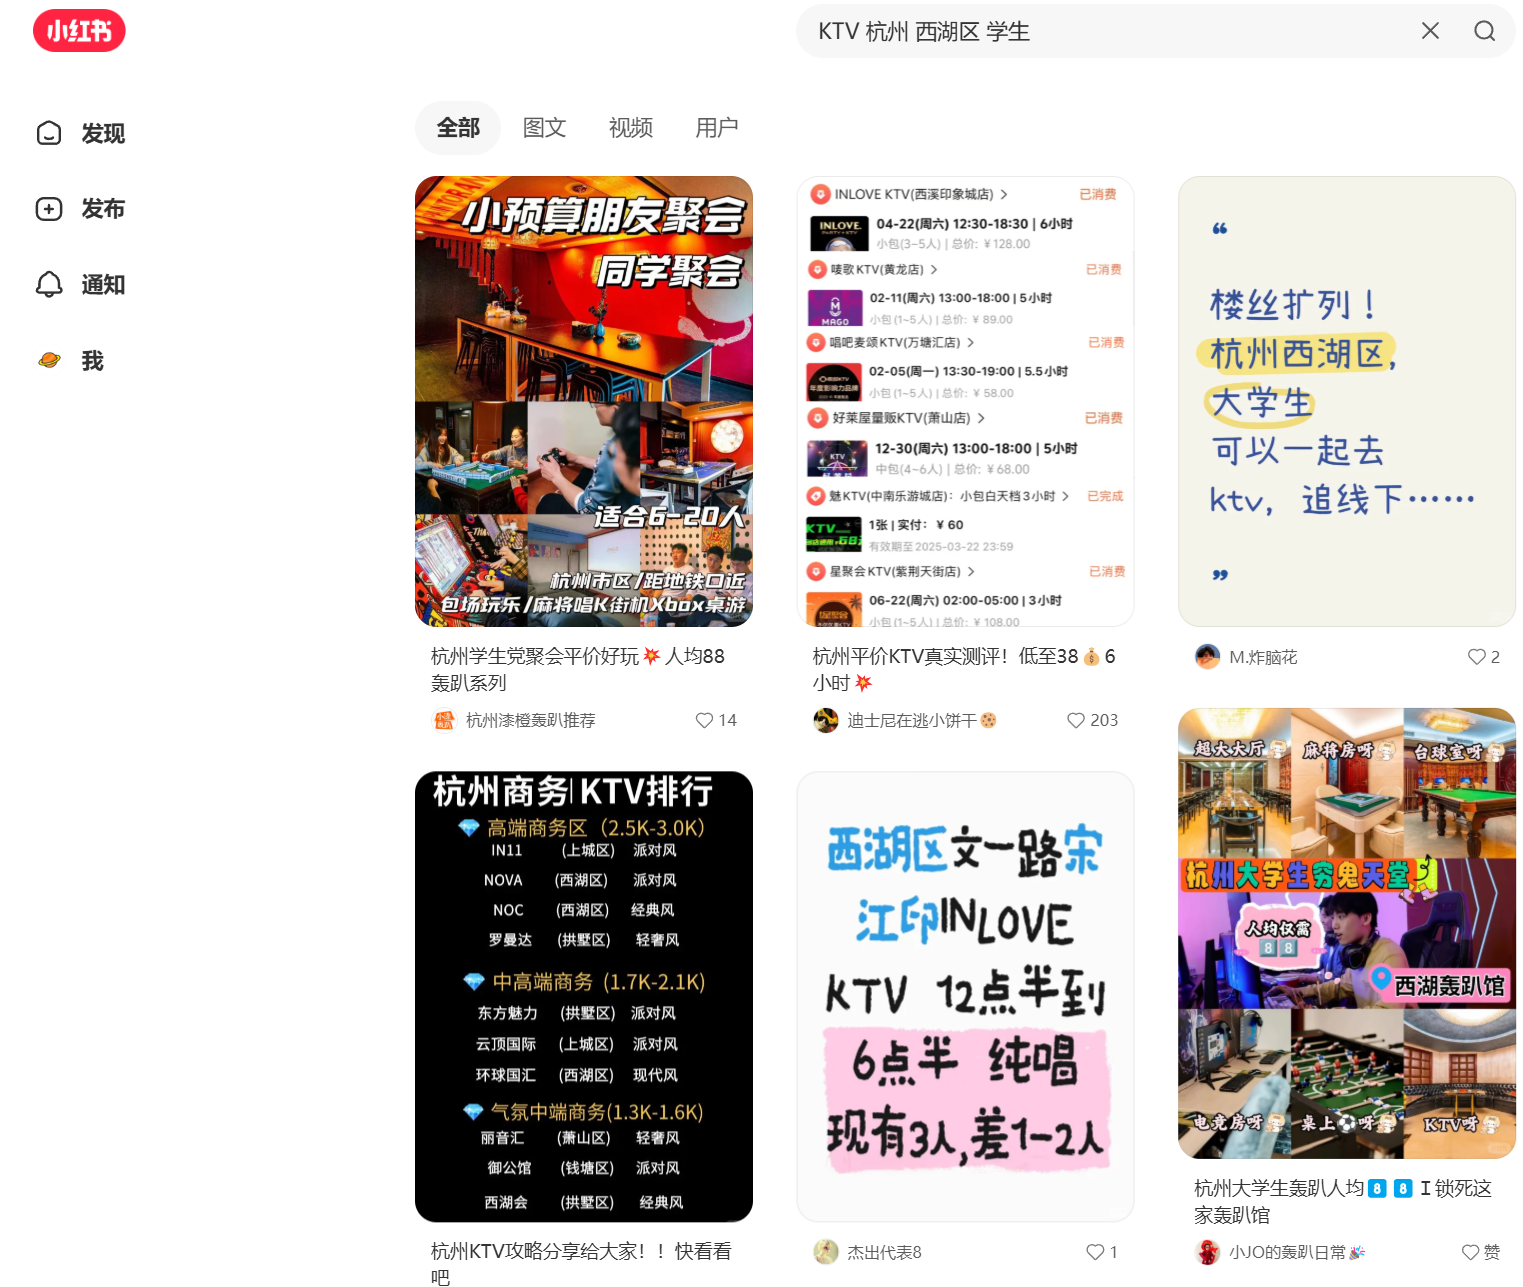
\includegraphics[width=.4\textwidth]{./figures/生活/ktv/1.png}
      \qquad
      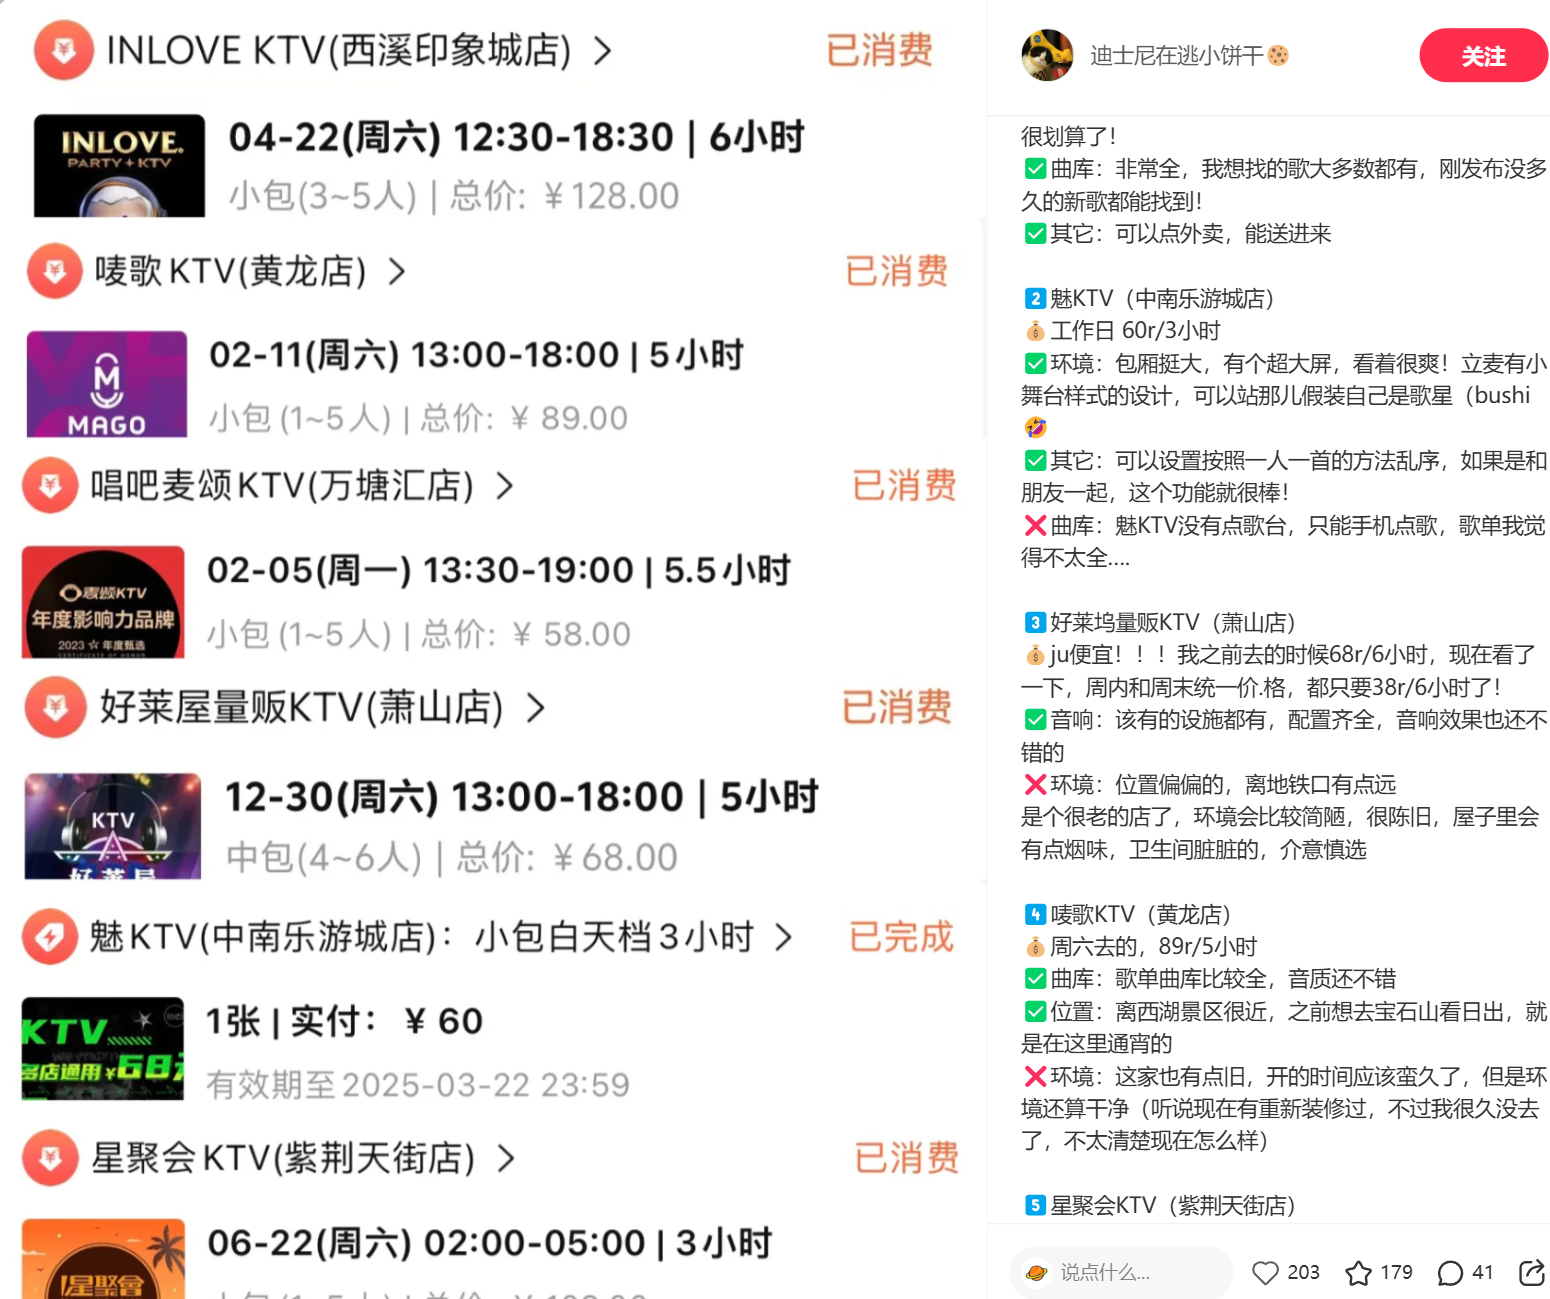
\includegraphics[width=.4\textwidth]{./figures/生活/ktv/2.png}
      \caption{小红书}
    \end{figure}

  \item 哔哩哔哩探店视频

  实景+测评查看(并关注点赞,收藏,转发数)

  寻求好评门店重叠

  \begin{figure}[H]
    \centering
    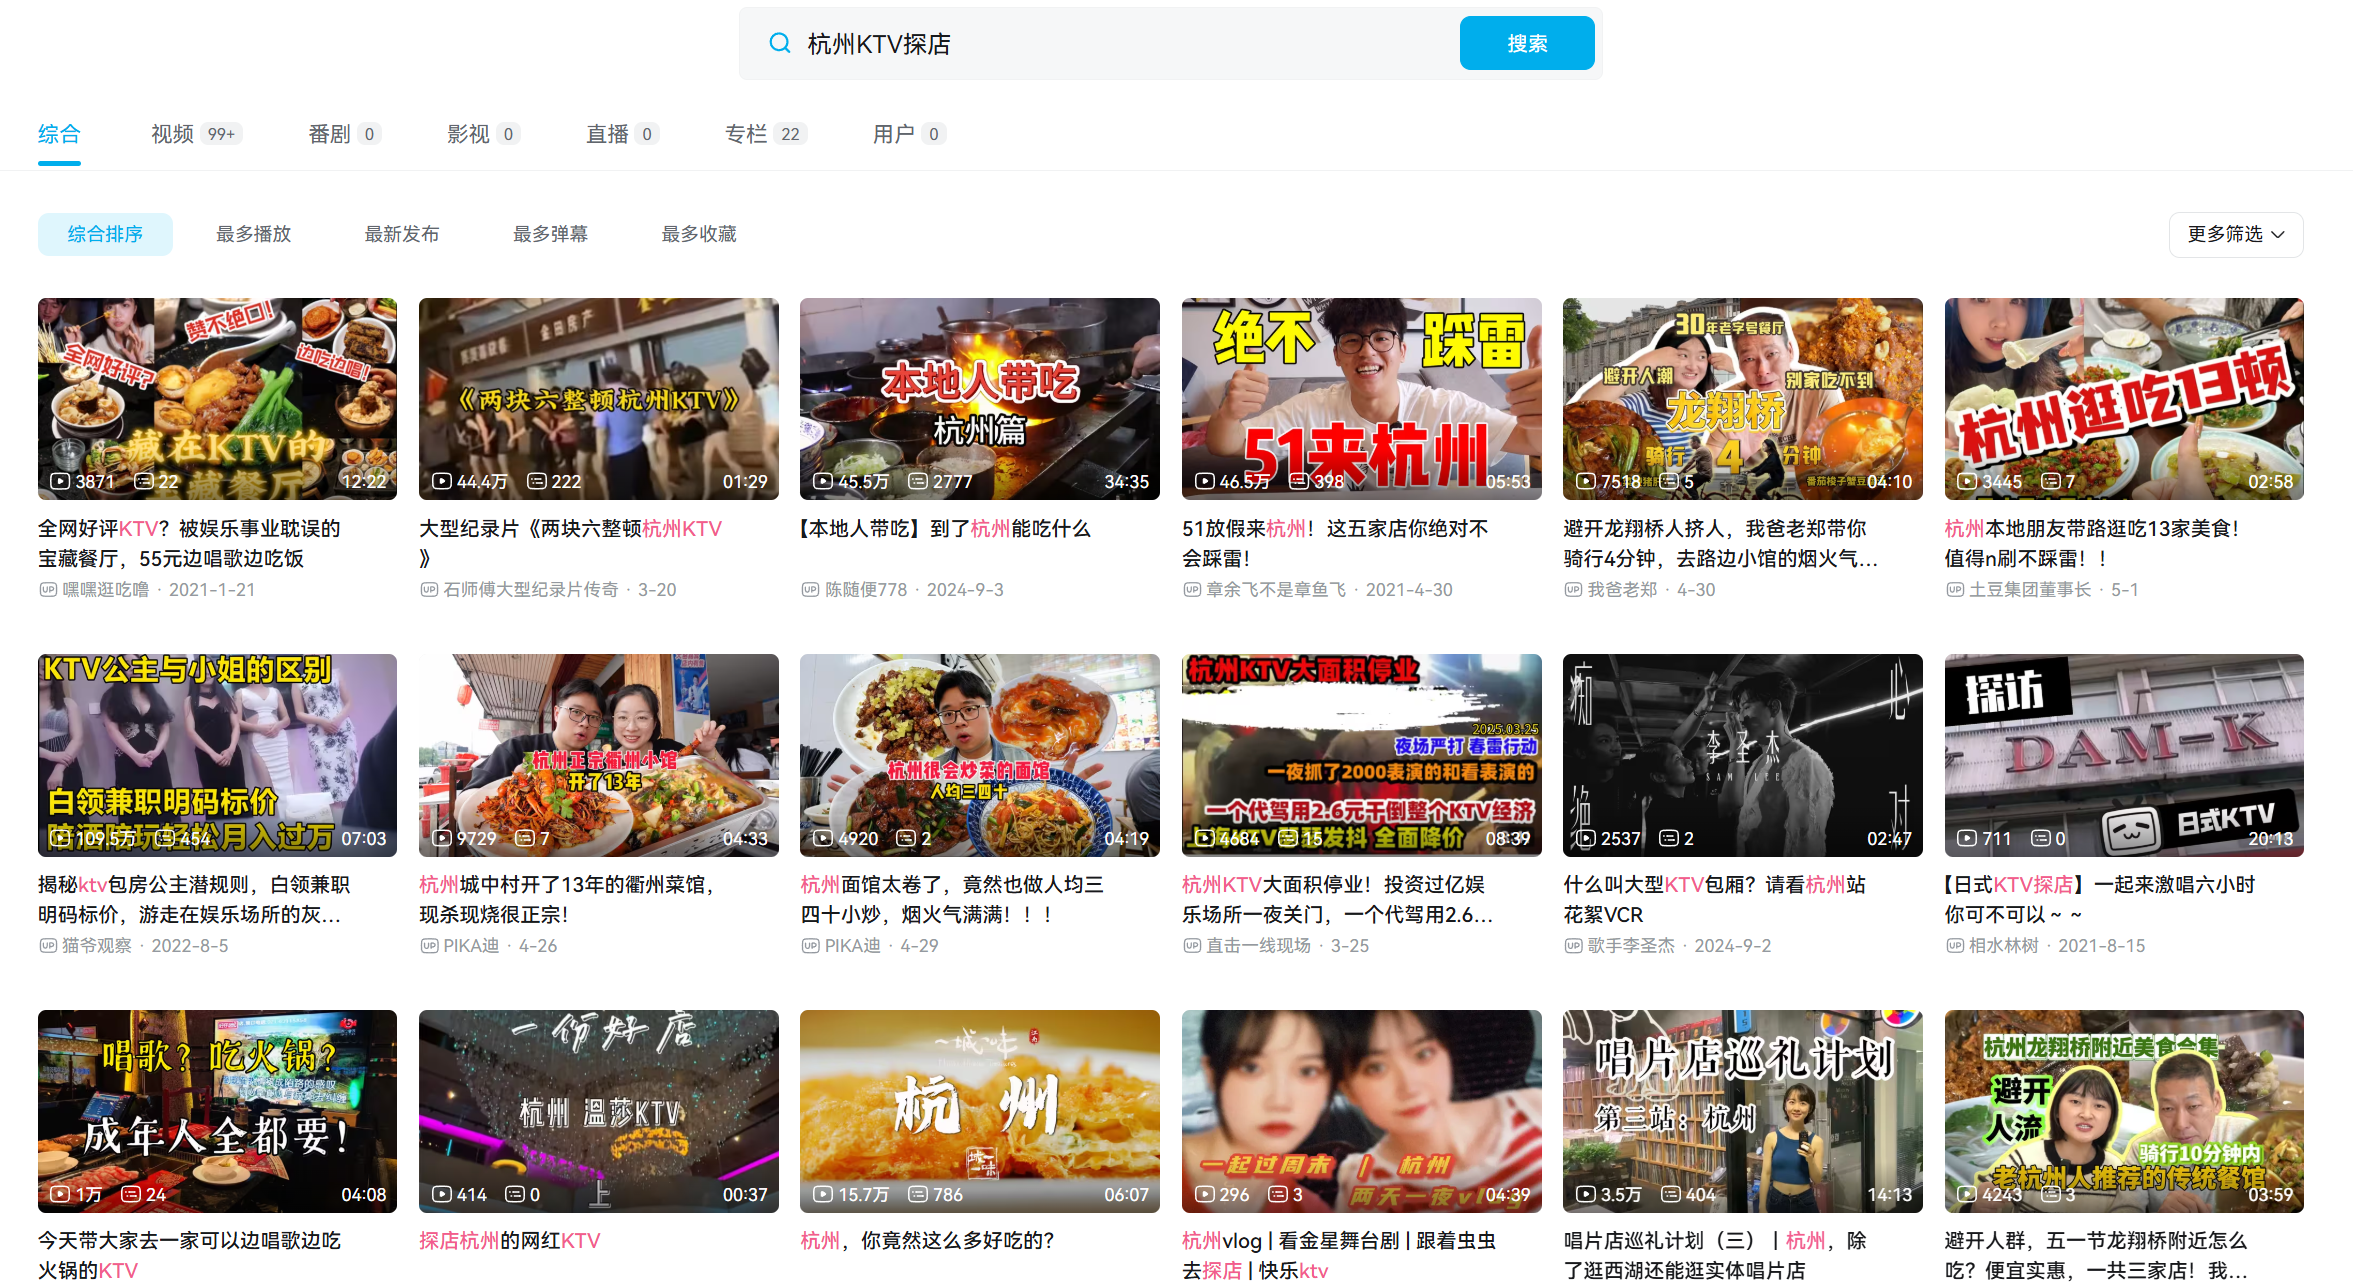
\includegraphics[width=.8\textwidth]{./figures/生活/ktv/bili.png}
    \caption{BiliBili}
  \end{figure}
  \item 美团搜索具体门店

  评分评论(重点关注差评率+差评理由,特别是卫生环境问题)+价格/门店信息查看+经营资质证明查看
  \begin{figure}[H]
    \centering
    
\includegraphics[width=.4\textwidth]{./figures/生活/ktv/m1.jpg}
    \qquad
    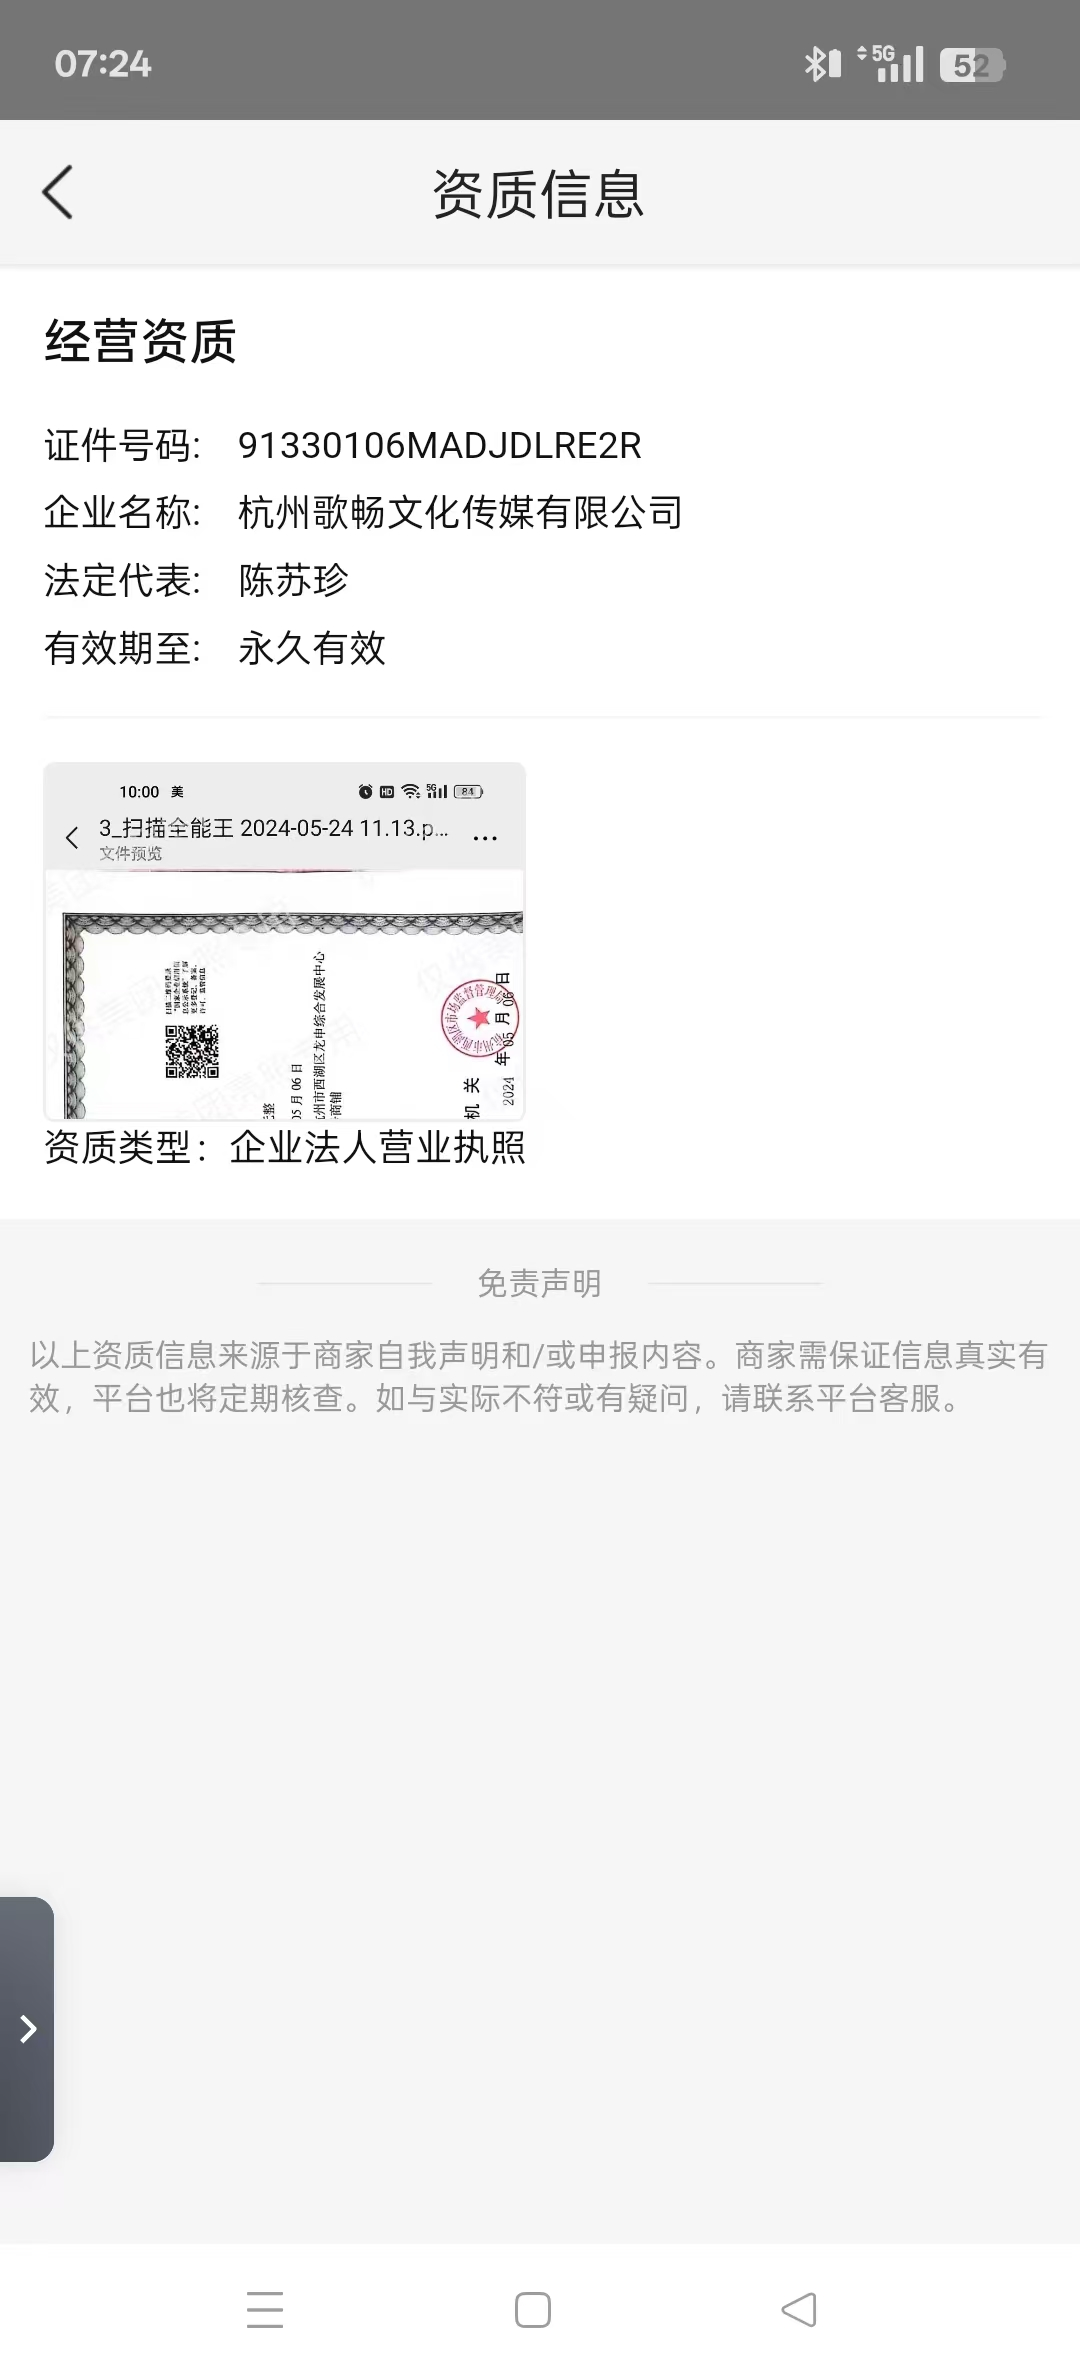
\includegraphics[width=.4\textwidth]{./figures/生活/ktv/m2.jpg}
    \caption{美团}
  \end{figure}
  \item 校友圈搜索相关体验回馈
  \begin{figure}[H]
    \centering
    
\includegraphics[width=.5\textwidth]{./figures/生活/ktv/d1.jpg}
    \caption{朵朵校友圈}
  \end{figure}
  \end{enumerate}
\end{exbox}
    \clearpage
    \chapter{线下活动}
    \label{activity}
    \section{宣传}
由同学制作好推文之后,我们在朋友圈,98,朵朵等平台转发和宣传了我们的\href{https://v.xiumi.us/board/v5/70Xhf/619220060}{推文}。
\begin{figure}[H]
\centering
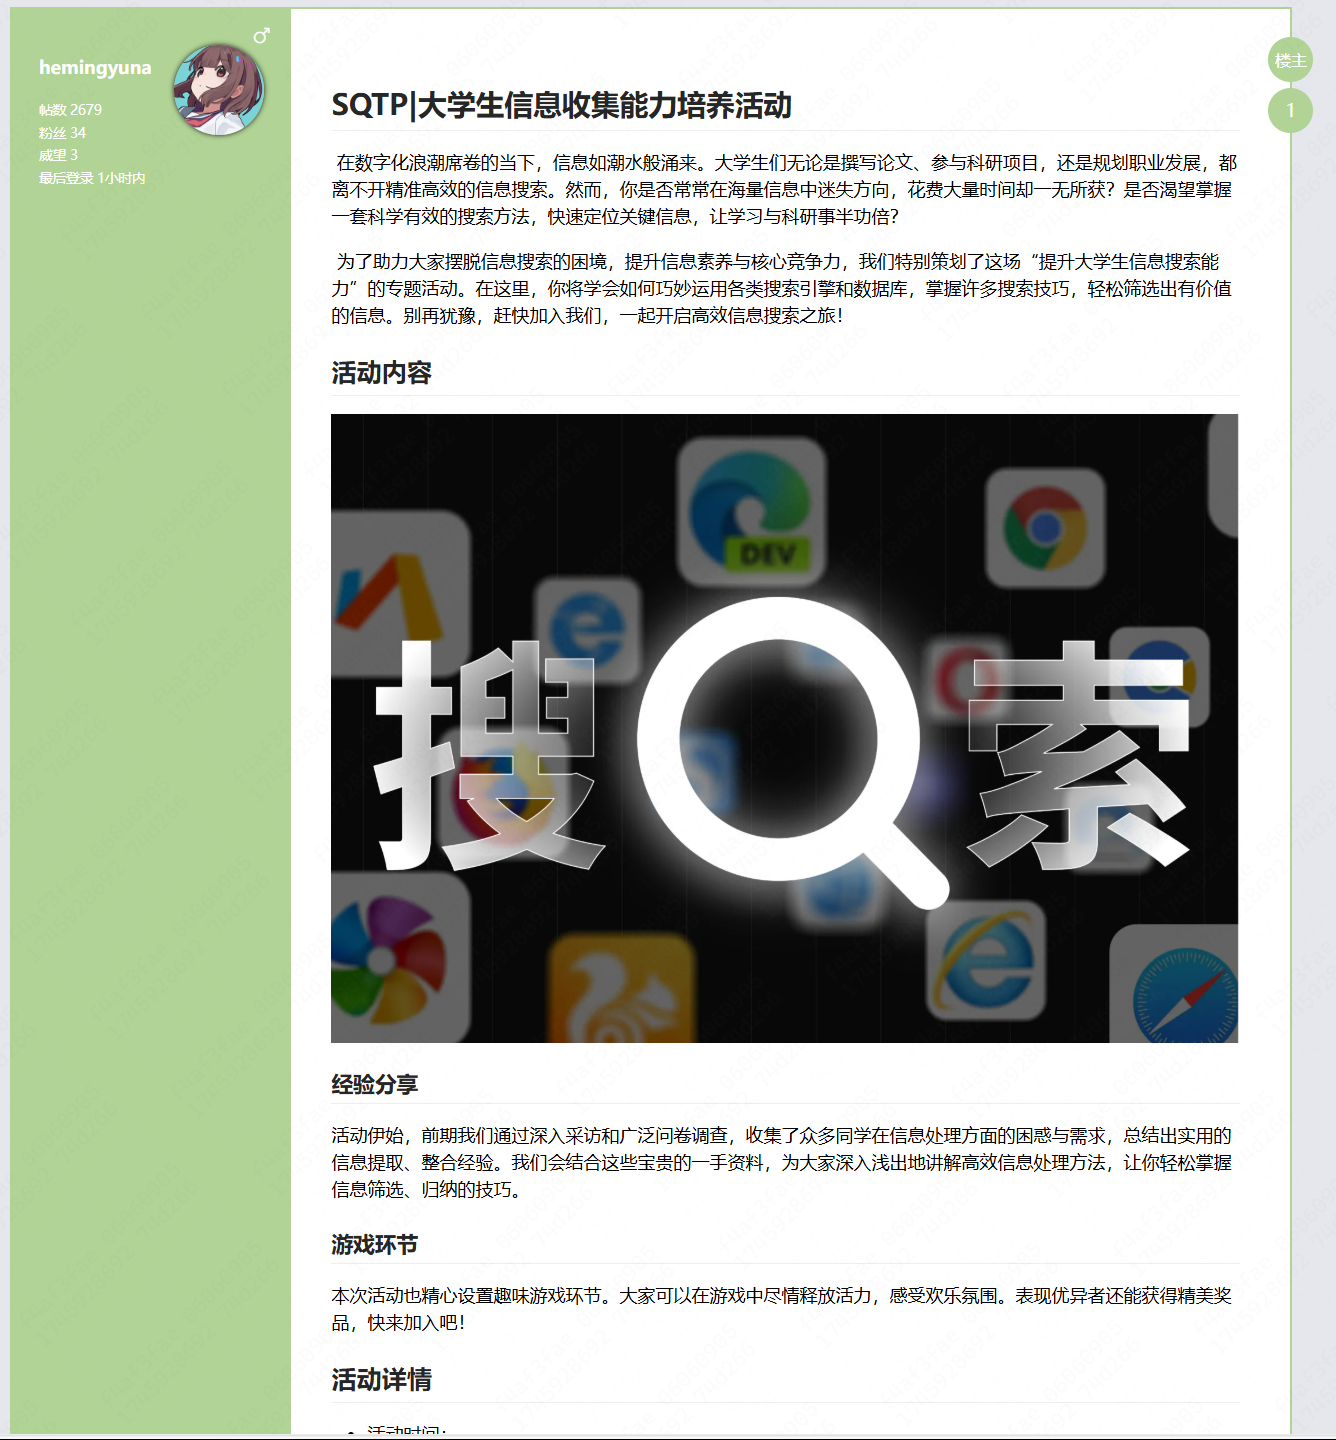
\includegraphics[width=.8\textwidth]{./figures/电脑端推文.png}

\includegraphics[width=.8\textwidth]{./figures/98宣传.png}
\caption{98推文及效果}
\end{figure}
\begin{figure}[H]
\centering

\includegraphics[width=.7\textwidth]{./resource/沙龙海报 .jpg}
\caption{活动海报}
\end{figure}
\section{宣讲会}
宣讲会基本按照手册编写顺序进行演讲,其中穿插了部分现场的案例演示与讲解。
\begin{figure}
    \centering
    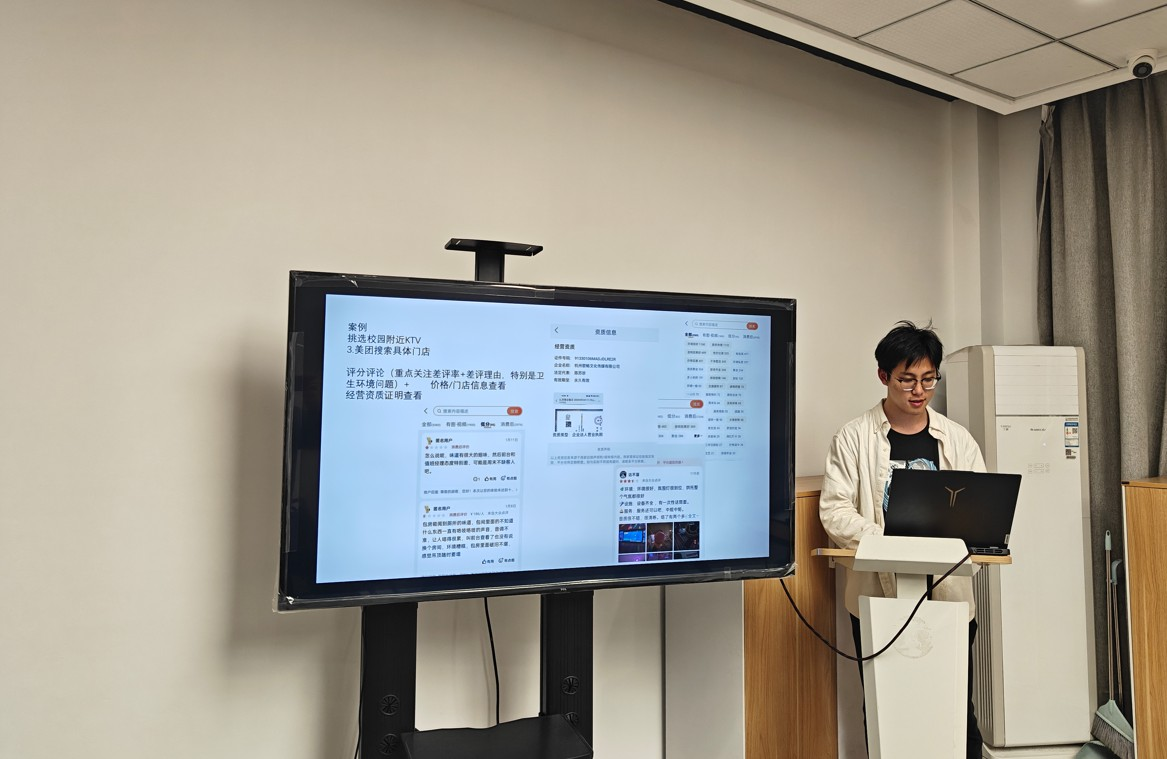
\includegraphics[width=.5\textwidth]{./figures/线下.jpg}
    \caption{线下宣讲}
\end{figure}
\section{网络迷踪信息搜索游戏}
\subsection{题目节选}
\begin{enumerate}
    \item 科研过程中遇到无法处理的实验数据时,会怎样处理
    \item 要写一篇课程论文,你会通过哪些途径完成你的论文
    \item 假如你是一个从未到过浙江大学的人,现在有一次机会可以来浙大游玩,你会怎样做攻略
    \item 你是一个不怎么会做饭的人,有一天爸妈都不在家,你又不想点外卖,会如何完成这顿饭的制作
    \item 突然电脑死机了,你会怎样解决这一问题
    \item 你和同学在某商城里寻找吃饭的地点。你会用什么途径寻找尽量好的餐厅?
    \item 3天后你就要大物小测了。你该如何寻找合适的复习资料?
    \item 允许使用电子设备搜索的课堂小测上,你该如何最快地找到尽可能对的答案?
    \item 选课时,你能列举3种获取课程信息的方式吗?
    \item 在qq等非正式平台看到了感兴趣的政治新闻,应该在哪里获取官方报道?
    \item 你准备保研,你应该去哪里查找上届保研录取分数?
\end{enumerate}
\begin{figure}
    \centering
    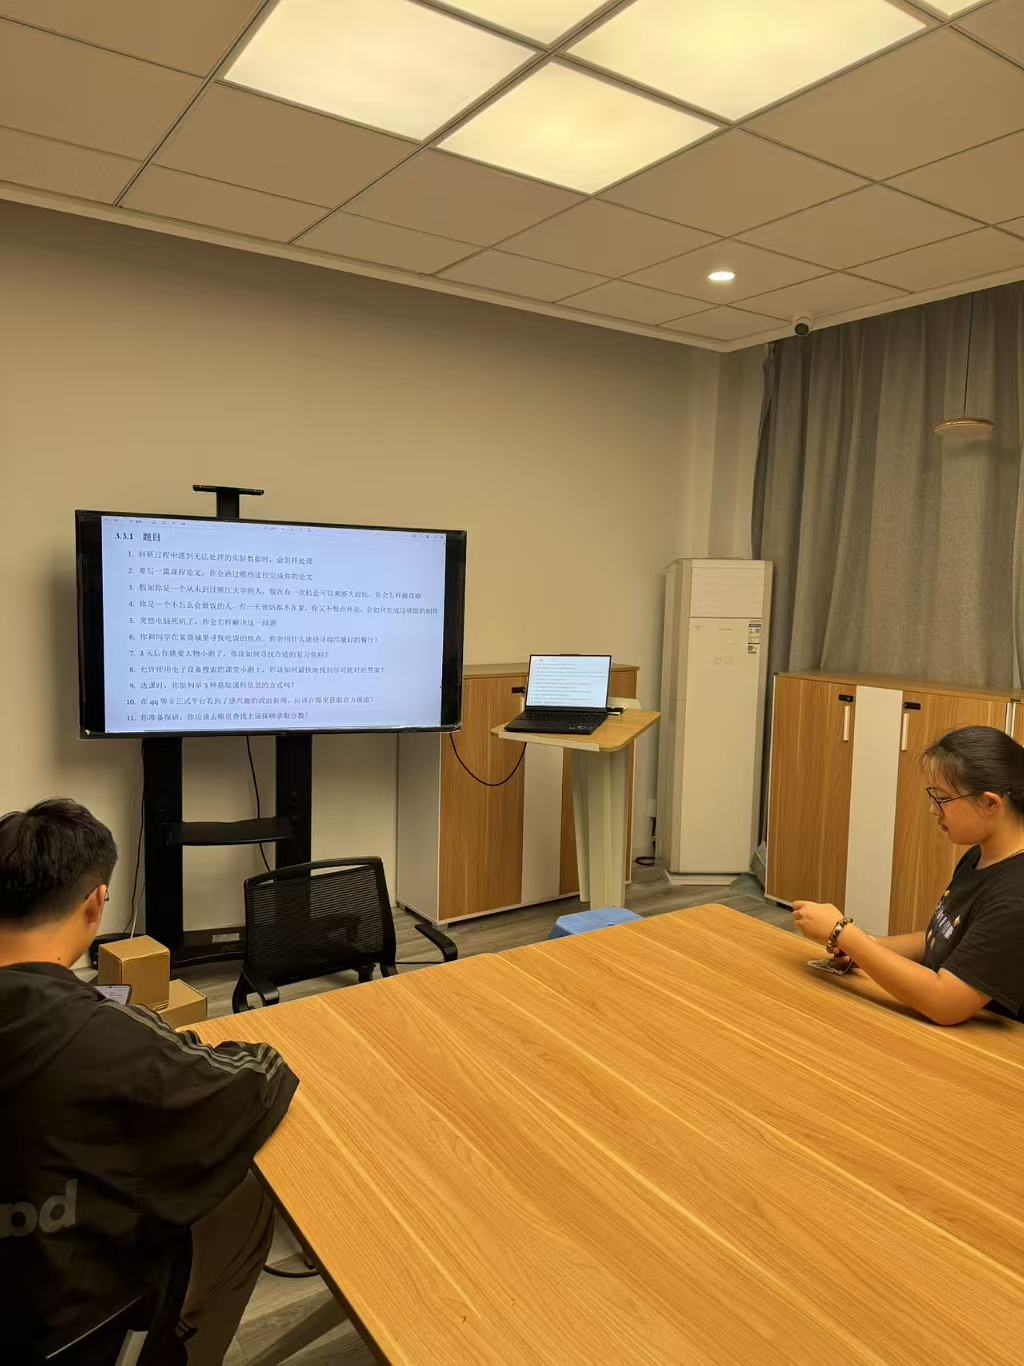
\includegraphics[width=.4\textwidth]{./figures/收集.jpg}
    \quad
    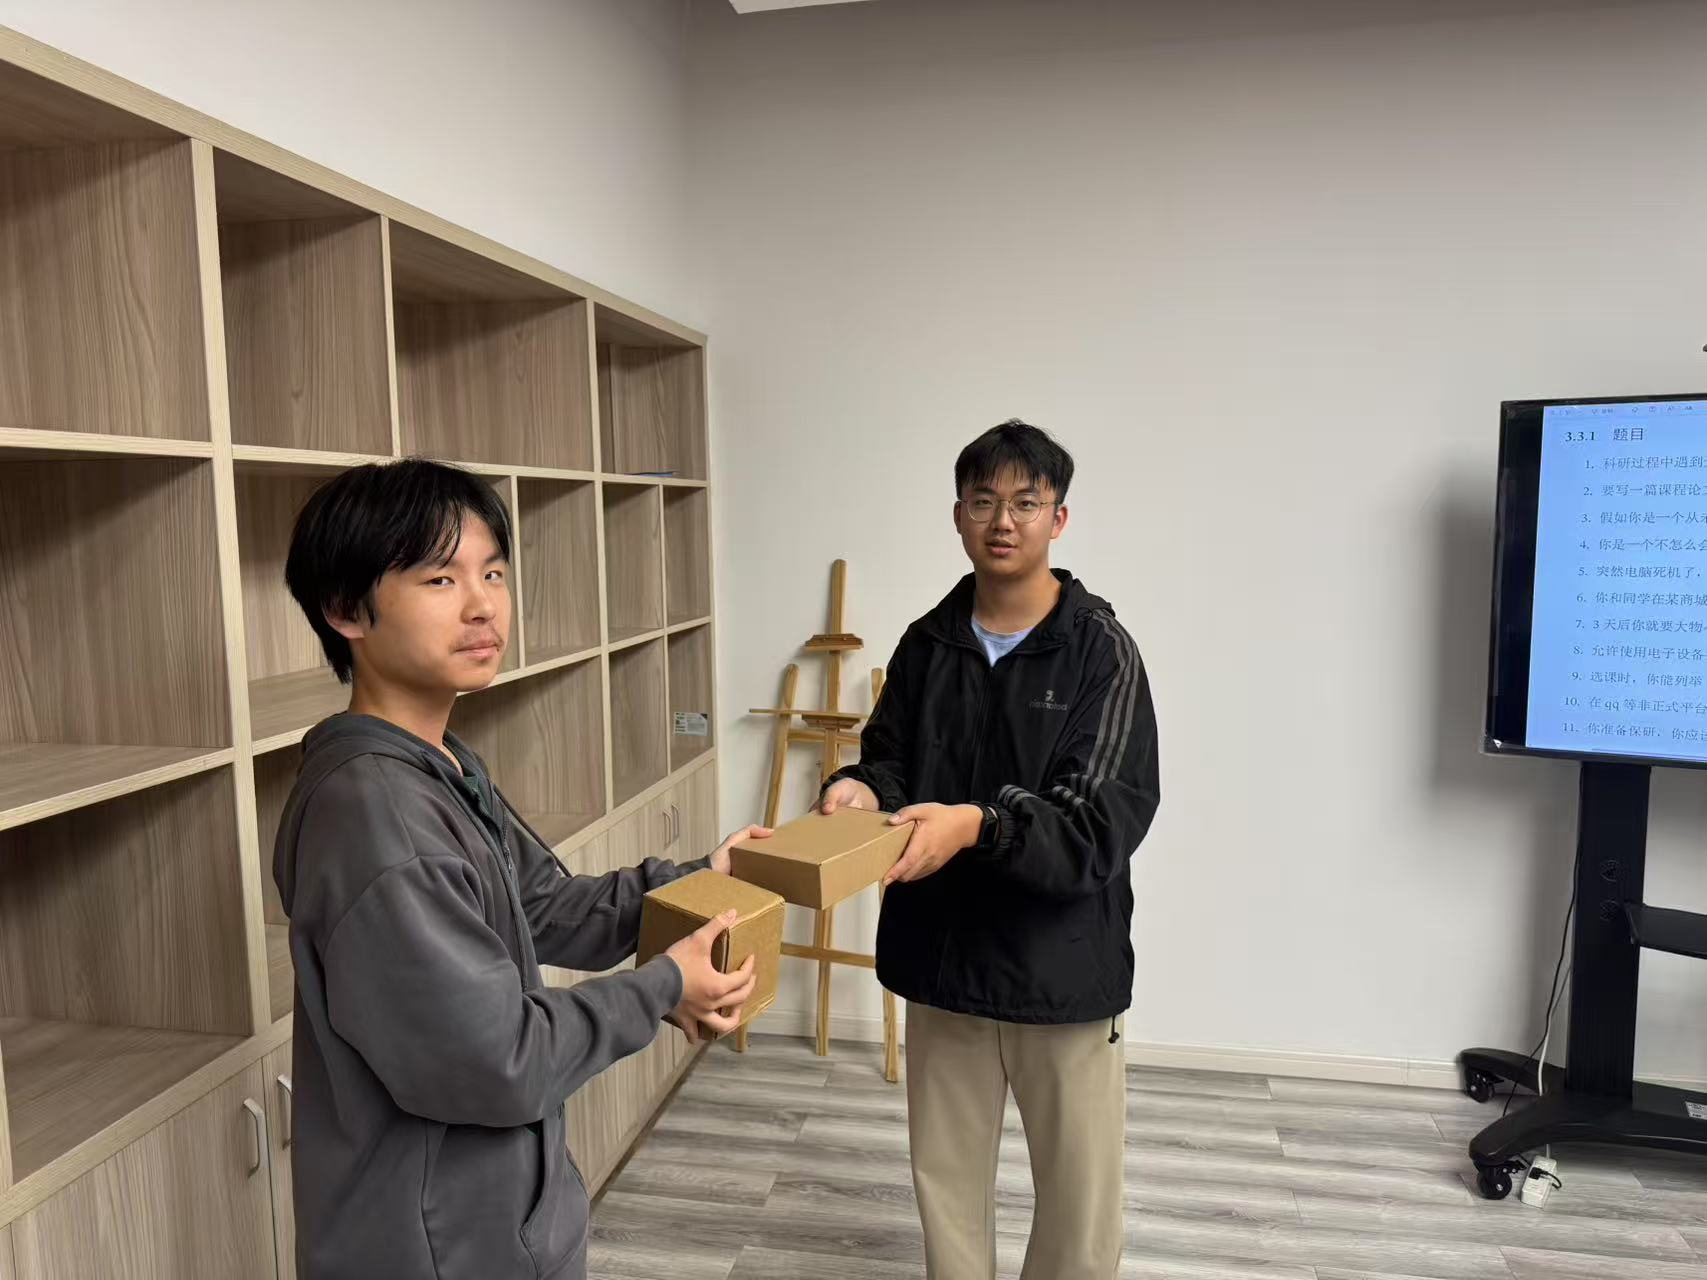
\includegraphics[width=.4\textwidth]{./figures/奖品发放.jpg}
    \caption{竞速信息收集与奖品发放}
\end{figure}
\subsection{反响}
关于``网络迷踪活动''同学们的反响:
\begin{notebox}
    ​参加网络迷踪游戏后,
    我深感这不仅是一场趣味横生的挑战,更是一次信息素养的实战演练。
    ​活动通过模拟真实的网络搜索场景,要求我们在海量信息中迅速提取有效线索,锻炼了我的观察力、逻辑思维和信息检索能力。
\end{notebox}
活动总结:

此次线下活动以“PPT宣讲会”与“网络迷踪信息搜索游戏”为核心,通过理论与实践结合的形式来提升大学生的信息检索能力与信息素养。
宣讲会围绕电子手册中科研、学习、生活三大场景的信息收集技巧展开,
结合案例演示与实时操作,深入解析关键词优化、数据库使用、多平台资源整合等方法,
帮助参与者构建结构化检索思维。
网络迷踪活动则创新性地将信息素养训练融入游戏机制,通过模拟真实搜索场景设计挑战题目,
要求参与者综合运用布尔逻辑检索等技巧,在限定时间内精准定位答案。
这种“寓教于乐”的形式不仅强化了理论知识的实际应用,还通过小礼品奖励机制激发参与热情,推动从被动接受信息到主动解决问题的思维转变。
    \clearpage
    \appendix
    \chapter{附录}
    \section{问卷原件}
    \begin{enumerate}[leftmargin=*]
    \item 你平时习惯在什么平台获取信息?
      \begin{enumerate}[label=\Alph*., itemsep=0pt]
        \item CC98
        \item 朵朵
        \item 视频平台(抖音、B站等)
        \item 百度
        \item 人工智能(ChatGPT、Kimi、豆包等)
        \item QQ 群
        \item 学长、学姐
        \item 舍友
        \item 同学
      \end{enumerate}

    \item 你平时都会搜寻哪些方面的信息?
      \begin{enumerate}[label=\Alph*., itemsep=0pt]
        \item 历年卷
        \item 题目解答
        \item 生活困惑
        \item 活动信息
        \item 情感问题
        \item 日常吃瓜
      \end{enumerate}

    \item 你在解决问题时会先搜索还是先向别人提问呢?
      \begin{enumerate}[label=\Alph*., itemsep=0pt]
        \item 搜索
        \item 提问
      \end{enumerate}

    \item 你认为你的搜索大多数时候与直接提问相比有效吗?
      \begin{enumerate}[label=\Alph*., itemsep=0pt]
        \item 是
        \item 否
      \end{enumerate}

    \item 你认为你自己信息搜索的能力足够吗?
      \begin{enumerate}[label=\Alph*., itemsep=0pt]
        \item 足够
        \item 不够
      \end{enumerate}

    \item 你认为自己信息搜索的能力对日常学习生活有影响吗?
      \begin{enumerate}[label=\Alph*., itemsep=0pt]
        \item 有
        \item 无
      \end{enumerate}

    \item 您认为大学生信息检索能力不足的原因有什么?(多选)
      \begin{enumerate}[label=\Alph*., itemsep=0pt]
        \item 缺少相关课程
        \item 学生兴趣不足
        \item 缺乏检索知识及相关技能
        \item 对电脑操作不够熟悉
        \item 其他
      \end{enumerate}

    \item 您认为以下哪些方式可提高大学生的信息检索能力?(多选)
      \begin{enumerate}[label=\Alph*., itemsep=0pt]
        \item 开设信息素养课程
        \item 举办信息素养讲座与培训
        \item 参加信息实践活动
        \item 阅读相关书籍
      \end{enumerate}

    \item 你的年龄
      \begin{enumerate}[label=\Alph*., itemsep=0pt]
        \item 18 岁以下
        \item 18–22 岁
        \item 22 岁以上
      \end{enumerate}

    \item 你使用信息检索的频率
      % 如需选项,可按上面格式添加

    \item 你知道一些信息检索的技巧(尤其是在浏览器上)吗?(比如使用 “-” 来排除结果)
      \begin{enumerate}[label=\Alph*., itemsep=0pt]
        \item 是
        \item 否
      \end{enumerate}

    \item 你是否有无法检索到想要的结果或者检索到弱相关的结果/广告的情况?
      \begin{enumerate}[label=\Alph*., itemsep=0pt]
        \item 经常
        \item 偶尔
        \item 几乎没有
        \item 没有
      \end{enumerate}

    \item 你是否会遇到在信息搜索上花费大量时间,却无法获得理想的资料?
      \begin{enumerate}[label=\Alph*., itemsep=0pt]
        \item 经常
        \item 偶尔
        \item 几乎没有
        \item 没有
      \end{enumerate}

    \item 你如何对搜索结果进行筛选?
      \begin{enumerate}[label=\Alph*., itemsep=0pt]
        \item 全部浏览
        \item 根据关键字吻合度
        \item 看点赞等热度数据
        \item 看过来人的评论
        \item 其他(请补充)
      \end{enumerate}

  \end{enumerate}

    \section{采访照片和提纲}
    \begin{enumerate}
    \item 当您需要完成课程论文时,第一反应是?\\
    完成课程论文是相对严谨专业的任务,在构思论文结构的同时还要适当引用前人的文章,故第一时间我会想到使用知网/万方等学术数据库。

    \item 你在找资料时最头疼的情况是?\\
    首先是很多情况下我都不确定自己搜的关键词对不对,有些搜索引擎对关键词要求极为苛刻,稍微有一点点偏差都可能导致搜索无果。还有很多专业术语让我迷惑,例如“现场总从线实时控制”之类。

    \item 你用过以下哪些“小技巧”?\\
    cc98 是校内极好的信息检索平台,速成论文小技巧我倒没搜索过,但在这上边能搜到很多精心写一篇论文的技能。至于拼接论文等不太光明磊落的技巧我是从未使用过。

    \item 如果让你教爸妈用手机查“大学奖学金怎么得”,你会?\\
    我会教他们先看短视频解说,再找文字版对照。现在的短视频覆盖领域极其广阔,且很多良心 up 主会非常认真的制作科普类视频,例如国奖获得经验分享的视频就有很多值得参考。

    \item 如果图书馆开设以下课程,你最想学什么?\\
    如今 AI 时代到来,如何用 AI 工具快速筛选文献(如 deepseek)助力自己很重要。我也想知道怎么从0到1搞定一篇文献综述,还有论文格式(查重规则与引用格式)相关内容。

    \item 你愿意参加哪种互助活动?\\
    可能是学长学姐的经验分享会吧,学长学姐是过来人,亲身经历更真实且有参考意义。或者说在 cc98 建立一个网站(或在 98 发帖),方便分析每门课的均绩等等,这种方式便捷高效。

    \item 你希望学校开发哪种神器?\\
    我超级希望能有根据课程自动推送参考资料的智能系统。

    \item 关于找资料,你最想吐槽的一句话:\\
    希望这世界上再也没有死板的关键词。

    \item 开学第一个月,你最抓狂的事是?\\
    $\checkmark$ 选课系统像中彩票

    \item 想查“如何不挂科”,你更信谁?\\
    $\checkmark$ 98 的学霸攻略,$\checkmark$ B站“三天突击高数”视频

    \item 【灵魂拷问】你用过以下哪种“野路子”搞资源?\\
    $\checkmark$ 98 跪求资料

    \item 如果学校推个“新生生存地图”,你最想要啥功能?\\
    $\checkmark$ 实时更新哪个食堂排队最短,$\checkmark$ 匿名评价选修课“水不水”,$\checkmark$ 全校 WiFi 信号强弱分布图,$\checkmark$ 一键呼叫学长学姐急救热线

    \item 你希望学校用哪种方式发通知?\\
    $\checkmark$ 宿舍楼下贴手绘漫画,$\checkmark$ 辅导员抖音直播唠嗑

\end{enumerate}

\begin{figure}[H]
    \centering
    
\includegraphics[width=\textwidth]{./resource/采访照片.JPG}
    \caption{线下采访照片}
\end{figure}
    % \section{推文}
    % 
\includepdf[pages={1-2}]{./resource/SQTP大学生信息收集能力培养活动.pdf}
    \section{感想与分工}
    \subsection{分工}
\begin{table}[H]
    \centering
    \caption{分工表}
    \begin{tabularx}{\textwidth}{>{\raggedright\arraybackslash}X >{\raggedright\arraybackslash}X}
      \toprule
      姓名  &   分工\\
      \midrule
        何铭源 &    确立项目,统筹策划,答辩,PPT修改,参与制定问卷并帮助投放,活动策划并组织,SQTP活动册整理和撰写\\
        严骏驰 &    采访及数据分析,辅助组织统筹,问卷投放,整理采访内容并对采访内容进行了分析,整理得出假新闻的识别与应对的一系列结论。\\
        何天佑 &    部分问卷设计,采访,活动海报设计,活动部分问题编写\\
        吴恩迪 &    推文制作,学习类资料搜集技巧\\
        池昊璞 &    部分问卷设计,部分问卷制作,投放与整理,搜索资料提出问题\\
        郑宇杰 &    11月开题答辩PPT制作,问卷投放,现场活动问题撰写,部分答辩PPT制作\\
        王弘晰 &    前期部分问卷设计,中期物资采购,后期资料整理(生活类部分),预约线下场地\\
        王俊凯 &    部分问卷设计,问卷制作,投放与整理,导出并分析问卷结果,整理知识点\\
        李泽楷 &    关于学生搜索现状的资料搜集,总结“理工类和社科类开题立项前的文献调研报告”\\
        唐焯奇 &    部分问卷设计,初期资料收集,负责总结信息收集整合相关方法 \\
      \bottomrule
    \end{tabularx}
  \end{table}
\subsection{感想}
何铭源:
\begin{notebox}
  从高中思维到大学思维的转变,对许多同学而言都是一道坎。小组作业中,总有部分同学习惯性地索要资料,而互联网上信息唾手可得的现状,更凸显了独立信息收集能力的重要性。因此,我们的SQTP项目聚焦于“信息收集与整合能力的培养”。

活动分为前期与后期。前期,我们广泛搜集相关资料,为后续工作指明方向。后期,我们创新性地借鉴游戏机制,旨在帮助同学们更快地接受“先搜索,再提问”的逻辑,并将我们整理出的信息收集方法融入日常学习。

作为项目的立项人,我肩负着活动策划和小组统筹的双重责任,这对我来说是一次极大的考验。完成整个SQTP后,我对信息收集,尤其是文献资料的搜集有了更深刻的理解。同时,在项目管理和活动策划方面,我的能力也得到了显著提升。
\end{notebox}
吴恩迪:
\begin{notebox}
  本次SQTP项目,围绕提升大学生搜索信息的能力展开,前期,我们进行了问卷投放、采访同学等工作,进行了初步的对同学们搜索信息的能力以及状况的了解,而后期,我们也根据获取的初步情况进行了活动的进一步展开。故而,在线下活动的展开之中,我们更加进一步的帮助同学们了解了更多所搜信息的渠道,全方面的对待这些渠道。此次活动的展开,不仅让我体会到了团队合作的魅力,也让我完善了信息搜索能力的方法知识,进一步提升了自我的能力品质。
\end{notebox}
王弘晰:
\begin{notebox}
  本次SQTP项目不知不觉走向了尾声。我为能参与其中,作出贡献感到自豪。

  此次项目聚焦于大一新生信息检索能力提升,我认为是非常贴合实际,有着巨大意义的。因为我自己检索能力也不突出,所以在项目的推进过程中,我也借此机会进行了广泛的调查和学习,在提升个人能力的同时也能够通过我们整理的资料去帮助身边的同学,这对于营造积极的学风与学习氛围有着正向影响,我想着也是学校组织,鼓励我们做SQTP项目的意义,也即在个人发展的同时促进集体的综合素养提升。

  值得一提的是,此次SQTP项目的目的和意义也与我作为班级学习委员的职责和使命高度吻合,也让我在工作过程中不断思考感悟,从而以更饱满的精神状态投入到学习和工作中。

  未来,我也将继续消化和运用本次项目中各成员做出的整理和分析,让这些技巧实打实地为我们的学习生活做出积极贡献。同时,项目的结题也不是为我们停止学习和推广画上句号,我们会吸取经验,并继续在相关领域做出努力和贡献。
\end{notebox}
李泽楷:
\begin{notebox}
  在完成小组调研任务的同时,我自己本身通过直播讲解获得了许多关于学术论文搜索的知识,
  并对学校图书馆的数据库、知网和搜索型AI等有了更多的了解,这会帮助我在以后的科研任务中更快速准确地获得我想要的资料,
  而这也是我想通过这次SQTP活动帮助同学们get到的技能,
  让同学们能更早更好地成为信息搜集者。
\end{notebox}
何天佑:
\begin{notebox}
  本次SQTP项目所调查的主题是大学生信息搜集方面的能力,这恰好是我在刚进入大学所欠缺的能力,
  因此,通过本次SQTP项目的进展,我不仅了解到大学生信息搜索能力的现状,而且还从中学到了很多获取信息的途径,
  不管是在日常生活上还是在学业科研方面,甚至是在休闲娱乐方面都让我有了很深的了解和经验,以及在项目进行过程中,
  结实了很多志同道合的伙伴,大家在一起工作的过程中互相帮助互相包容,锻炼了我团队协作能力和沟通交流的能力。
  总而言之,这次项目经历让我受益匪浅,希望可以与同学们一起参加更多的项目。
\end{notebox}
郑宇杰:
\begin{notebox}
  \begin{enumerate}
    \item 提问时要结合自身生活实际。问题涵盖面要广,体现出主题的同时也要保证一定的趣味性。
    \item 善于利用搜索工具和网络社区,寻找更广泛人群更普遍的问题。
  \end{enumerate}
\end{notebox}
严骏驰:
\begin{notebox}
  我们组聚焦于信息检索能力提升,整合了生活学习科研等多方面的信息搜集技巧。
  并通过线下分享会等形式传播我们的研究成果,既帮助大家填充了一些检索领域的空白,又帮助我们自身提升综合检索能力,受益匪浅。
\end{notebox}
池昊璞:
\begin{notebox}
  参与项目前,我以为信息检索不过是输入关键词的简单操作,直到真正设计采访提纲时,才意识到系统性检索的难度——如何精准定位冷门资料、辨别信息真伪都是学问。后期搜索资料设计问卷过程中也暴露了问题,比如我曾误抄一整段的AI文献,但后来发现直接大段摘录简直八竿子打不着。最触动的还是后面团队互助、经验传承的细节:感觉什么都没干时,何天佑为我指点迷津,差点忘记发感悟时,严骏驰委婉的和我讲,被检索式困住时,也有学长提醒“用限定词缩小范围”,这些零散的经验传递比教程更有效。唯一遗憾的是,许多实践中摸索出的非常规检索路径未被系统记录,若能整理成案例库或许更有价值。
\end{notebox}
    \section{时间线}
    \begin{figure}[H]
        \centering
        \begin{tikzpicture}[
        node distance=2cm,
        activity/.style={draw, rounded corners, align=center, inner sep=0.2cm},
        time/.style={below=0.3cm of #1, align=center},
        arrow/.style={-Latex}
        ]
      \node (title) [activity] {前期准备工作};
      \node (t_title) [time=title] {11月月初至月中};

      \node (survey) [activity, right=of title] {问卷设计};
      \node (t_survey) [time=survey] {11月初及三月初};

      \node (defense) [activity, right=of survey] {答辩};
      \node (t_defense) [time=defense] {11月中};

      \node (purchase) [activity, right=of defense] {物资采购};
      \node (t_purchase) [time=purchase] {2月中};

      \node (interview) [activity, below=1.5cm of purchase, xshift=-4cm] {采访及数据分析};
      \node (t_interview) [time=interview] {3月初};

      \node (share) [activity, right=of interview] {分享会};
      \node (t_share) [time=share] {4-5月};

      \draw [arrow] (title) -- (survey);
      \draw [arrow] (survey) -- (defense);
      \draw [arrow] (defense) -- (purchase);
      \draw [arrow] (purchase) -- (interview);
      \draw [arrow] (interview) -- (share);

    \end{tikzpicture}
    \caption{项目进行时间线}
    \end{figure}
    \clearpage
\end{document}
